%%%%%%%%%%%%%%%%%%%%%%%%%%%%% Thesis.tex %%%%%%%%%%%%%%%%%%%%%%%%%%%%%%%
%                                                                      %
%  ---------- Master of Science Dissertation template ----------       %
%                                                                      %
%  Template for the Master Thesis according to the regulations         %
%  published by the Academic Board (Direcção Académica) at IST.        %
%                                                                      %
%  For an up-to-date guide, please refer to the official website          %
%  http://academica.tecnico.ulisboa.pt/alunos/dissertacao-de-mestrado/ %
%                                                                      %
%       Andre C. Marta                                                 %
%       Area Cientifica de Mecanica Aplicada e Aeroespacial            %
%       Departamento de Engenharia Mecanica                            %
%       Instituto Superior Tecnico                                     %
%       Av. Rovisco Pais                                               %
%       1049-001 Lisboa                                                %
%       Portugal                                                       %
%       Tel: +351 21 841 9469                                          %
%                        3469 (extension)                              %
%       Email: andre.marta@tecnico.ulisboa.pt                          %
%                                                                      %
%  Created:       Jan 20, 2011                                         %
%  Last Modified: Feb 19, 2018                                         %
%                                                                      %
%%%%%%%%%%%%%%%%%%%%%%%%%%%%%%%%%%%%%%%%%%%%%%%%%%%%%%%%%%%%%%%%%%%%%%%%
%  Revision history                                                    %
%  v1 - 2011/01/24 - original template                                 %
%  v2 - 2012/10/30 - new IST image and glossary support                %
%  v3 - 2013/12/10 - update according to 2012/13 official guide        %
%  v4 - 2014/02/28 - new default for bibliography style                %
%  v5 - 2014/05/07 - update according to 2013/14 official guide        %
%  v6 - 2015/07/02 - cover page format fixed,                          %
%                    contents page numbering fixed,                    %
%                    better language support,                          %
%                    enhanced examples of tables,                      %
%                    new option for appendix page numbering format,    %
%                    custom bibliography style                         %
%  v7 - 2018/02/19 - multiple citations compressed                     %
%%%%%%%%%%%%%%%%%%%%%%%%%%%%%%%%%%%%%%%%%%%%%%%%%%%%%%%%%%%%%%%%%%%%%%%%
%                                                                      %
% To generate the PDF file, type "make" at the terminal prompt.        %
%                                                                      %
% The IST template LaTeX package was created by the author             %
% and it can be downloaded from:                                       %
% https://fenix.ist.utl.pt/homepage/ist31052/                          %
%                                                                      %
% The external packages can be downloaded from                         %
% the Comprehensive TeX Archive Network at http://www.ctan.org/        %
%                                                                      %
% List of LaTex symbols:                                               %
% http://www.ctan.org/tex-archive/info/symbols/comprehensive/          %
%                                                                      %
% Help with LaTex can be found at                                      %
% http://www.giss.nasa.gov/tools/latex/ltx-2.html                      %
% http://en.wikibooks.org/wiki/LaTeX                                   %
%%%%%%%%%%%%%%%%%%%%%%%%%%%%%%%%%%%%%%%%%%%%%%%%%%%%%%%%%%%%%%%%%%%%%%%%

%%%%%%%%%%%%%%%%%%%%%%%%%%%%%%%%%%%%%%%%%%%%%%%%%%%%%%%%%%%%%%%%%%%%%%%%
%     Preamble                                                         %
%%%%%%%%%%%%%%%%%%%%%%%%%%%%%%%%%%%%%%%%%%%%%%%%%%%%%%%%%%%%%%%%%%%%%%%%

% ----------------------------------------------------------------------
%  Set the document class
% ----------------------------------------------------------------------
\documentclass[10pt,a4paper,twoside]{report}

\usepackage{listings}
\usepackage{color}
\usepackage[printonlyused]{acronym}
\usepackage[all]{nowidow}
\usepackage{titlesec}

\setcounter{secnumdepth}{4}

\titleformat{\paragraph}
{\normalfont\normalsize\bfseries}{\theparagraph}{1em}{}
\titlespacing*{\paragraph}
{0pt}{3.25ex plus 1ex minus .2ex}{1.5ex plus .2ex}



\definecolor{dkgreen}{rgb}{0,0.6,0}
\definecolor{gray}{rgb}{0.5,0.5,0.5}
\definecolor{mauve}{rgb}{0.58,0,0.82}

\lstset{frame=tb,
	language=C,
	aboveskip=5mm,
	belowskip=5mm,
	showstringspaces=false,
	columns=flexible,
	basicstyle={\small\ttfamily},
	numbers=none,
	numberstyle=\tiny\color{gray},
	keywordstyle=\color{blue},
	commentstyle=\color{dkgreen},
	stringstyle=\color{mauve},
	breaklines=true,
	breakatwhitespace=true,
	tabsize=2,
}


% ----------------------------------------------------------------------
% Define external packages, language, margins, fonts, and new commands
% ----------------------------------------------------------------------
%%%%%%%%%%%%%%%%%%%%%%%%%%%%%%%%%%%%%%%%%%%%%%%%%%%%%%%%%%%%%%%%%%%%%%%%
%                                                                      %
%     File: Thesis_Preamble.tex                                        %
%     Tex Master: Thesis.tex                                           %
%                                                                      %
%     Author: Andre C. Marta                                           %
%     Last modified : 9 Apr 2015                                       %
%                                                                      %
%%%%%%%%%%%%%%%%%%%%%%%%%%%%%%%%%%%%%%%%%%%%%%%%%%%%%%%%%%%%%%%%%%%%%%%%

% ----------------------------------------------------------------------
% Define document language.
% ----------------------------------------------------------------------

% 'inputenc' package
%
% Accept different input encodings.
% http://www.ctan.org/tex-archive/macros/latex/base/
%
% > allows typing non-english text in LaTeX sources.
%
% ******************************* SELECT *******************************
%\usepackage[latin1]{inputenc} % <<<<< Windows
\usepackage[utf8]{inputenc}   % <<<<< Linux
% ******************************* SELECT *******************************


% 'babel' package
%
% Multilingual support for Plain TeX or LaTeX.
% http://www.ctan.org/tex-archive/macros/latex/required/babel/
%
% > sets the variable names according to the language selected
%
% ******************************* SELECT *******************************
%\usepackage[portuguese]{babel} % <<<<< Portuguese
\usepackage[english]{babel} % <<<<< English
% ******************************* SELECT *******************************


% List of LaTeX variable names: \abstractname, \appendixname, \bibname,
%   \chaptername, \contentsname, \listfigurename, \listtablename, ...)
% http://www.tex.ac.uk/cgi-bin/texfaq2html?label=fixnam
%
% Changing the words babel uses (uncomment and redefine as necessary...)
%
\newcommand{\acknowledgments}{@undefined} % new LaTeX variable name
%
% > English
%
\addto\captionsenglish{\renewcommand{\acknowledgments}{Acknowledgments}}
%\addto\captionsenglish{\renewcommand{\contentsname}{Contents}}
%\addto\captionsenglish{\renewcommand{\listtablename}{List of Tables}}
%\addto\captionsenglish{\renewcommand{\listfigurename}{List of Figures}}
%\addto\captionsenglish{\renewcommand{\nomname}{Nomenclature}}
%\addto\captionsenglish{\renewcommand{\glossaryname}{Glossary}}
%\addto\captionsenglish{\renewcommand{\acronymname}{List of Acronyms}}
%\addto\captionsenglish{\renewcommand{\bibname}{References}} % Bibliography
%\addto\captionsenglish{\renewcommand{\appendixname}{Appendix}}

% > Portuguese
%
\addto\captionsportuguese{\renewcommand{\acknowledgments}{Agradecimentos}}
%\addto\captionsportuguese{\renewcommand{\contentsname}{Conte\'{u}do}}
%\addto\captionsportuguese{\renewcommand{\listtablename}{Lista de Figuras}}
%\addto\captionsportuguese{\renewcommand{\listfigurename}{Lista de Tabelas}}
\addto\captionsportuguese{\renewcommand{\nomname}{Lista de S\'{i}mbolos}} % Nomenclatura
%\addto\captionsportuguese{\renewcommand{\glossary}{Gloss\'{a}rio}}
%\addto\captionsportuguese{\renewcommand{\acronymname}{Lista de Abrevia\c{c}\~{o}es}}
%\addto\captionsportuguese{\renewcommand{\bibname}{Refer\^{e}ncias}} % Bibliografia
%\addto\captionsportuguese{\renewcommand{\appendixname}{Anexo}} % Apendice


% ----------------------------------------------------------------------
% Define cover fields in both english and portuguese.
% ----------------------------------------------------------------------
%
\newcommand{\coverThesis}{@undefined} % new LaTeX variable name
\newcommand{\coverSupervisors}{@undefined} % new LaTeX variable name
\newcommand{\coverExaminationCommittee}{@undefined} % new LaTeX variable name
\newcommand{\coverChairperson}{@undefined} % new LaTeX variable name
\newcommand{\coverSupervisor}{@undefined} % new LaTeX variable name
\newcommand{\coverMemberCommittee}{@undefined} % new LaTeX variable name
% > English
\addto\captionsenglish{\renewcommand{\coverThesis}{Thesis to obtain the Master of Science Degree in}}
\addto\captionsenglish{\renewcommand{\coverSupervisors}{Supervisor(s)}}
\addto\captionsenglish{\renewcommand{\coverExaminationCommittee}{Examination Committee}}
\addto\captionsenglish{\renewcommand{\coverChairperson}{Chairperson}}
\addto\captionsenglish{\renewcommand{\coverSupervisor}{Supervisor}}
\addto\captionsenglish{\renewcommand{\coverMemberCommittee}{Member of the Committee}}
% > Portuguese
\addto\captionsportuguese{\renewcommand{\coverThesis}{Disserta\c{c}\~{a}o para obten\c{c}\~{a}o do Grau de Mestre em}}
\addto\captionsportuguese{\renewcommand{\coverSupervisors}{Orientador(es)}}
\addto\captionsportuguese{\renewcommand{\coverExaminationCommittee}{J\'{u}ri}}
\addto\captionsportuguese{\renewcommand{\coverChairperson}{Presidente}}
\addto\captionsportuguese{\renewcommand{\coverSupervisor}{Orientador}}
\addto\captionsportuguese{\renewcommand{\coverMemberCommittee}{Vogal}}


% ----------------------------------------------------------------------
% Define default and cover page fonts.
% ----------------------------------------------------------------------

% Use Arial font as default
%
\renewcommand{\rmdefault}{phv}
\renewcommand{\sfdefault}{phv}

% Define cover page fonts
%
%         encoding     family       series      shape
%  \usefont{T1}     {phv}=helvetica  {b}=bold    {n}=normal
%                   {ptm}=times      {m}=normal  {sl}=slanted
%                                                {it}=italic
% see more examples at
% http://julien.coron.free.fr/languages/latex/fonts/
%
\def\FontLn{% 16 pt normal
  \usefont{T1}{phv}{m}{n}\fontsize{16pt}{16pt}\selectfont}
\def\FontLb{% 16 pt bold
  \usefont{T1}{phv}{b}{n}\fontsize{16pt}{16pt}\selectfont}
\def\FontMn{% 14 pt normal
  \usefont{T1}{phv}{m}{n}\fontsize{14pt}{14pt}\selectfont}
\def\FontMb{% 14 pt bold
  \usefont{T1}{phv}{b}{n}\fontsize{14pt}{14pt}\selectfont}
\def\FontSn{% 12 pt normal
  \usefont{T1}{phv}{m}{n}\fontsize{12pt}{12pt}\selectfont}


% ----------------------------------------------------------------------
% Define page margins and line spacing.
% ----------------------------------------------------------------------

% 'geometry' package
%
% Flexible and complete interface to document dimensions.
% http://www.ctan.org/tex-archive/macros/latex/contrib/geometry/
%
% > set the page margins (2.5cm minimum in every side, as per IST rules)
%
\usepackage{geometry}	
\geometry{verbose,tmargin=2.5cm,bmargin=2.5cm,lmargin=2.5cm,rmargin=2.5cm}

% 'setspace' package
%
% Set space between lines.
% http://www.ctan.org/tex-archive/macros/latex/contrib/setspace/
%
% > allow setting line spacing (line spacing of 1.5, as per IST rules)
%
\usepackage{setspace}
\renewcommand{\baselinestretch}{1.5}


% ----------------------------------------------------------------------
% Include external packages.
% Note that not all of these packages may be available on all system
% installations. If necessary, include the .sty files locally in
% the <jobname>.tex file directory.
% ----------------------------------------------------------------------

% 'graphicx' package
%
% Enhanced support for graphics.
% http://www.ctan.org/tex-archive/macros/latex/required/graphics/
%
% > extends arguments of the \includegraphics command
%
\usepackage{graphicx}


% 'color' package
%
% Colour control for LaTeX documents.
% http://www.ctan.org/tex-archive/macros/latex/required/graphics/
%
% > defines color macros: \color{<color name>}
%
%\usepackage{color}


% 'amsmath' package
%
% Mathematical enhancements for LaTeX.
% http://www.ctan.org/tex-archive/macros/latex/required/amslatex/
%
% > American Mathematical Society plain Tex macros
%
\usepackage{amsmath}  % AMS mathematical facilities for LaTeX.
\usepackage{amsthm}   % Typesetting theorems (AMS style).
\usepackage{amsfonts} % 


% 'wrapfig' package
%
% Produces figures which text can flow around.
% http://www.ctan.org/tex-archive/macros/latex/contrib/wrapfig/
%
% > wrap figures/tables in text (i.e., Di Vinci style)
%
% \usepackage{wrapfig}


% 'subfigure' package
%
% Deprecated: Figures divided into subfigures.
% http://www.ctan.org/tex-archive/obsolete/macros/latex/contrib/subfigure/
%
% > subcaptions for subfigures
%
\usepackage{subfigure}


% 'subfigmat' package
%
% Automates layout when using the subfigure package.
% http://www.ctan.org/tex-archive/macros/latex/contrib/subfigmat/
%
% > matrices of similar subfigures
%
\usepackage{subfigmat}


% 'url' package
%
% Verbatim with URL-sensitive line breaks.
% http://www.ctan.org/tex-archive/macros/latex/contrib/url/
%
% > URLs in BibTex
%
% \usepackage{url}


% 'varioref' package
%
% Intelligent page references.
% http://www.ctan.org/tex-archive/macros/latex/required/tools/
%
% > smart page, figure, table and equation referencing
%
%\usepackage{varioref}


% 'dcolumn' package
%
% Align on the decimal point of numbers in tabular columns.
% http://www.ctan.org/tex-archive/macros/latex/required/tools/
%
% > decimal-aligned tabular math columns
%
\usepackage{dcolumn}
\newcolumntype{d}{D{.}{.}{-1}} % column aligned by the point separator '.'
\newcolumntype{e}{D{E}{E}{-1}} % column aligned by the exponent 'E'


% 'verbatim' package
%
% Reimplementation of and extensions to LaTeX verbatim.
% http://www.ctan.org/tex-archive/macros/latex/required/tools/
%
% > provides the verbatim environment (\begin{verbatim},\end{verbatim})
%   and a comment environment (\begin{comment},  \end{comment})
%
% \usepackage{verbatim}


% 'moreverb' package
%
% Extended verbatim.
% http://www.ctan.org/tex-archive/macros/latex/contrib/moreverb/
%
% > supports tab expansion and line numbering
%
% \usepackage{moreverb}



% 'nomencl' package
%
% Produce lists of symbols as in nomenclature.
% http://www.ctan.org/tex-archive/macros/latex/contrib/nomencl/
%
% The nomencl package makes use of the MakeIndex program
% in order to produce the nomenclature list.
%
% Nomenclature
% 1) On running the file through LATEX, the command \makenomenclature
%    in the preamble instructs it to create/open the nomenclature file
%    <jobname>.nlo corresponding to the LATEX file <jobname>.tex and
%    writes the information from the \nomenclature commands to this file.
% 2) The next step is to invoke MakeIndex in order to produce the
%    <jobname>.nls file. This can be achieved by making use of the
%    command: makeindex <jobname>.nlo -s nomencl.ist -o <jobname>.nls
% 3) The last step is to invoke LATEX on the <jobname>.tex file once
%    more. There, the \printnomenclature in the document will input the
%    <jobname>.nls file and process it according to the given options.
%
% http://www-h.eng.cam.ac.uk/help/tpl/textprocessing/nomencl.pdf
%
% Nomenclature (produces *.nlo *.nls files)
\usepackage{nomencl}
\makenomenclature
%
% Group variables according to their symbol type
%
\RequirePackage{ifthen} 
\ifthenelse{\equal{\languagename}{english}}%
    { % English
    \renewcommand{\nomgroup}[1]{%
      \ifthenelse{\equal{#1}{R}}{%
        \item[\textbf{Roman symbols}]}{%
        \ifthenelse{\equal{#1}{G}}{%
          \item[\textbf{Greek symbols}]}{%
          \ifthenelse{\equal{#1}{S}}{%
            \item[\textbf{Subscripts}]}{%
            \ifthenelse{\equal{#1}{T}}{%
              \item[\textbf{Superscripts}]}{}}}}}%
    }{% Portuguese
    \renewcommand{\nomgroup}[1]{%
      \ifthenelse{\equal{#1}{R}}{%
        \item[\textbf{Simbolos romanos}]}{%
        \ifthenelse{\equal{#1}{G}}{%
          \item[\textbf{Simbolos gregos}]}{%
          \ifthenelse{\equal{#1}{S}}{%
            \item[\textbf{Subscritos}]}{%
            \ifthenelse{\equal{#1}{T}}{%
              \item[\textbf{Sobrescritos}]}{}}}}}%
    }%


% 'glossary' package
%
% Create a glossary.
% http://www.ctan.org/tex-archive/macros/latex/contrib/glossary/
%
% Glossary (produces *.glo *.ist files)
\usepackage[number=none]{glossary}
% (remove blank line between groups)
\setglossary{gloskip={}}
% (redefine glossary style file)
%\renewcommand{\istfilename}{myGlossaryStyle.ist}
\makeglossary


% 'rotating' package
%
% Rotation tools, including rotated full-page floats.
% http://www.ctan.org/tex-archive/macros/latex/contrib/rotating/
%
% > show wide figures and tables in landscape format:
%   use \begin{sidewaystable} and \begin{sidewaysfigure}
%   instead of 'table' and 'figure', respectively.
%
\usepackage{rotating}


% 'hyperref' package
%
% Extensive support for hypertext in LaTeX.
% http://www.ctan.org/tex-archive/macros/latex/contrib/hyperref/
%
% > Extends the functionality of all the LATEX cross-referencing
%   commands (including the table of contents, bibliographies etc) to
%   produce \special commands which a driver can turn into hypertext
%   links; Also provides new commands to allow the user to write adhoc
%   hypertext links, including those to external documents and URLs.
%
\usepackage[pdftex]{hyperref} % enhance documents that are to be
                              % output as HTML and PDF
\hypersetup{colorlinks,       % color text of links and anchors,
                              % eliminates borders around links
%            linkcolor=red,    % color for normal internal links
            linkcolor=black,  % color for normal internal links
            anchorcolor=black,% color for anchor text
%            citecolor=green,  % color for bibliographical citations
            citecolor=black,  % color for bibliographical citations
%            filecolor=magenta,% color for URLs which open local files
            filecolor=black,  % color for URLs which open local files
%            menucolor=red,    % color for Acrobat menu items
            menucolor=black,  % color for Acrobat menu items
%            pagecolor=red,    % color for links to other pages
            pagecolor=black,  % color for links to other pages
%            urlcolor=cyan,    % color for linked URLs
            urlcolor=black,   % color for linked URLs
	          bookmarks=true,         % create PDF bookmarks
	          bookmarksopen=false,    % don't expand bookmarks
	          bookmarksnumbered=true, % number bookmarks
	          pdftitle={Thesis},
            pdfauthor={Andre C. Marta},
            pdfsubject={Thesis Title},
            pdfkeywords={Thesis Keywords},
            pdfstartview=FitV,
            pdfdisplaydoctitle=true}


% 'hypcap' package
%
% Adjusting the anchors of captions.
% http://www.ctan.org/tex-archive/macros/latex/contrib/oberdiek/
%
% > fixes the problem with hyperref, that links to floats points
%   below the caption and not at the beginning of the float.
%
\usepackage[figure,table]{hypcap}


% 'natbib' package
%
% Flexible bibliography support.
% http://www.ctan.org/tex-archive/macros/latex/contrib/natbib/
%
% > produce author-year style citations
%
% \citet  and \citep  for textual and parenthetical citations, respectively
% \citet* and \citep* that print the full author list, and not just the abbreviated one
% \citealt is the same as \citet but without parentheses. Similarly, \citealp is \citep without parentheses
% \citeauthor
% \citeyear
% \citeyearpar
%
%% natbib options can be provided when package is loaded \usepackage[options]{natbib}
%%
%% Following options are valid:
%%
%%   round  -  round parentheses are used (default)
%%   square -  square brackets are used   [option]
%%   curly  -  curly braces are used      {option}
%%   angle  -  angle brackets are used    <option>
%%   semicolon  -  multiple citations separated by semi-colon (default)
%%   colon  - same as semicolon, an earlier confusion
%%   comma  -  separated by comma
%%   authoryear - for author–year citations (default)
%%   numbers-  selects numerical citations
%%   super  -  numerical citations as superscripts, as in Nature
%%   sort   -  sorts multiple citations according to order in ref. list
%%   sort&compress   -  like sort, but also compresses numerical citations
%%   compress - compresses without sorting
%%
% ******************************* SELECT *******************************
%\usepackage{natbib}          % <<<<< References in alphabetical list Correia, Silva, ...
\usepackage[numbers,sort&compress]{natbib} % <<<<< References in numbered list [1],[2],...
% ******************************* SELECT *******************************
\usepackage{listings}

% 'notoccite' package
%
% Prevent trouble from citations in table of contents, etc.
% http://ctan.org/pkg/notoccite
%
% > If you have \cite com­mands in \sec­tion-like com­mands, or in \cap­tion,
%   the ci­ta­tion will also ap­pear in the ta­ble of con­tents, or list of what­ever.
%   If you are also us­ing an un­srt-like bib­li­og­ra­phy style, these ci­ta­tions will
%   come at the very start of the bib­li­og­ra­phy, which is con­fus­ing. This pack­age
%   sup­presses the ef­fect.
%
\usepackage{notoccite}


% 'multirow' package
%
% Create tabular cells spanning multiple rows
% http://www.ctan.org/pkg/multirow
%
\usepackage{multirow}


% 'booktabs' package
%
% Publication quality tables in LaTeX
% http://www.ctan.org/pkg/booktabs
%
% > en­hance the qual­ity of ta­bles in LaTeX, pro­vid­ing ex­tra com­mands.
%
% \renewcommand{\arraystretch}{<ratio>} % space between rows
%
\usepackage{booktabs}
%\newcommand{\ra}[1]{\renewcommand{\arraystretch}{#1}}


% 'pdfpages' package
%
% Include PDF documents in LaTeX
% http://www.ctan.org/pkg/pdfpages
%
% > in­clu­sion of ex­ter­nal multi-page PDF doc­u­ments in LaTeX doc­u­ments.
%   Pages may be freely se­lected and sim­i­lar to psnup it is pos­si­ble to put
%   sev­eral log­i­cal pages onto each sheet of pa­per.
%
% \includepdf{filename.pdf}
% \includepdf[pages={4-9},nup=2x3,landscape=true]{filename.pdf}
%
\usepackage{pdfpages}


% ----------------------------------------------------------------------
% Define new commands to assure consistent treatment throughout document
% ----------------------------------------------------------------------

\newcommand{\ud}{\mathrm{d}}                % total derivative
\newcommand{\degree}{\ensuremath{^\circ\,}} % degrees

% Abbreviations

\newcommand{\mcol}{\multicolumn}            % table format

\newcommand{\eqnref}[1]{(\ref{#1})}
\newcommand{\class}[1]{\texttt{#1}}
\newcommand{\package}[1]{\texttt{#1}}
\newcommand{\file}[1]{\texttt{#1}}
\newcommand{\BibTeX}{\textsc{Bib}\TeX}

% Typefaces ( example: {\bf Bold text here} )
%
% > pre-defined
%   \bf % bold face
%   \it % italic
%   \tt % typewriter
%
% > newly defined
\newcommand{\tr}[1]{{\ensuremath{\textrm{#1}}}}   % text roman
\newcommand{\tb}[1]{{\ensuremath{\textbf{#1}}}}   % text bold face
\newcommand{\ti}[1]{{\ensuremath{\textit{#1}}}}   % text italic
\newcommand{\mc}[1]{{\ensuremath{\mathcal{#1}}}}  % math calygraphy
\newcommand{\mco}[1]{{\ensuremath{\mathcalold{#1}}}}% math old calygraphy
\newcommand{\mr}[1]{{\ensuremath{\mathrm{#1}}}}   % math roman
\newcommand{\mb}[1]{{\ensuremath{\mathbf{#1}}}}   % math bold face
\newcommand{\bs}[1]{\ensuremath{\boldsymbol{#1}}} % math symbol
\def\bm#1{\mathchoice                             % math bold
  {\mbox{\boldmath$\displaystyle#1$}}%
  {\mbox{\boldmath$#1$}}%
  {\mbox{\boldmath$\scriptstyle#1$}}%
  {\mbox{\boldmath$\scriptscriptstyle#1$}}}
\newcommand{\boldcal}[1]{{\ensuremath{\boldsymbol{\mathcal{#1}}}}}% math bold calygraphy

 % file "Thesis_Preamble.tex"

%%%%%%%%%%%%%%%%%%%%%%%%%%%%%%%%%%%%%%%%%%%%%%%%%%%%%%%%%%%%%%%%%%%%%%%%
%     Begin Document                                                   %
%%%%%%%%%%%%%%%%%%%%%%%%%%%%%%%%%%%%%%%%%%%%%%%%%%%%%%%%%%%%%%%%%%%%%%%%
\begin{document}

% Set plain page style (no headers, footer with centered page number)
\pagestyle{plain}

% Set Roman numbering (i,ii,...) before the start of chapters
\pagenumbering{roman}

% ----------------------------------------------------------------------
%  Cover page
% ----------------------------------------------------------------------
%%%%%%%%%%%%%%%%%%%%%%%%%%%%%%%%%%%%%%%%%%%%%%%%%%%%%%%%%%%%%%%%%%%%%%%%
%                                                                      %
%     File: Thesis_FrontCover.tex                                      %
%     Tex Master: Thesis.tex                                           %
%                                                                      %
%     Author: Andre C. Marta                                           %
%     Last modified :  2 Jul 2015                                      %
%                                                                      %
%%%%%%%%%%%%%%%%%%%%%%%%%%%%%%%%%%%%%%%%%%%%%%%%%%%%%%%%%%%%%%%%%%%%%%%%

\thispagestyle {empty}

% IST Logo - Signature A
% parameters: bb=llx lly urx ury (bounding box), width=h_length, height=v_length, angle=angle, scale=factor, clip=true/false, draft=true/false. 

\includegraphics[bb=9.5cm 11cm 0cm 0cm,scale=0.29]{IST_A_CMYK_POS}

\begin{center}
%
% Figure (Image or plot)
\vspace{2.5cm}
% height = 50 mm
%\includegraphics[height=50mm]{Figures/Airbus_A350.jpg}

% Title, author and degree
\vspace{1.0cm}
{\FontLb Deep Neural Network on the Versat Reconfigurable Processor} \\ % <<<<< EDIT TITLE
%\vspace{0.2cm}
%{\FontMn Subtitle (optional)} \\
%\vspace{1.9cm}
\vspace{2.6cm}
{\FontMb João Pedro Costa Luís Cardoso} \\ % <<<<< EDIT NAME
\vspace{2.0cm}

{\FontSn \coverThesis} \\
\vspace{0.3cm}
{\FontLb Electrical and Computer Engineering} \\ % <<<<< EDIT COURSE
\vspace{1.0cm}
{\FontSn %
\begin{tabular}{ll}
 \coverSupervisors: Prof. José João Henriques Teixeira de Sousa \\ % <<<<< EDIT NAME
               % <<<<< EDIT NAME
\end{tabular} } \\
\vspace{1.0cm}
\vspace{0.3cm}
{\FontSn %
\begin{tabular}{c}
%\coverChairperson:     Prof. Full Name          \\ % <<<<< EDIT NAME
%\coverSupervisor:      Prof. José João Henriques Teixeira de Sousa \\ % <<<<< EDIT NAME
%\coverMemberCommittee: TO ADD           % <<<<< EDIT NAME
\end{tabular} } \\
\vspace{1.5cm}
{\FontMb September 2022} \\ % <<<<< EDIT DATE (corresponds to date of oral examination)
%
\end{center}

%\coverExaminationCommittee % file "Thesis_FrontCover.tex"
\cleardoublepage


% ----------------------------------------------------------------------
%  Declaration
% ----------------------------------------------------------------------
\section*{Declaration}
I declare that this document is an original work of my own authorship and that it 
fulfills all the requirements of the Code of Conduct and Good Practices of the 
Universidade de Lisboa.
\cleardoublepage


% ----------------------------------------------------------------------
% Dedication page (optional)
% ----------------------------------------------------------------------

%%%%%%%%%%%%%%%%%%%%%%%%%%%%%%%%%%%%%%%%%%%%%%%%%%%%%%%%%%%%%%%%%%%%%%%%
%                                                                      %
%     File: Thesis_Dedication.tex                                      %
%     Tex Master: Thesis.tex                                           %
%                                                                      %
%     Author: Andre C. Marta                                           %
%     Last modified :  2 Jul 2015                                      %
%                                                                      %
%%%%%%%%%%%%%%%%%%%%%%%%%%%%%%%%%%%%%%%%%%%%%%%%%%%%%%%%%%%%%%%%%%%%%%%%

\null\vskip5cm%
\begin{flushright}
     Dedicated to my fiancée Matilde and my firstborn son Francisco.
\end{flushright}
\vfill\newpage

 % file "Thesis_Dedication.tex"
\cleardoublepage

% ----------------------------------------------------------------------
%  Acknowledgments (optional)
% ----------------------------------------------------------------------
%%%%%%%%%%%%%%%%%%%%%%%%%%%%%%%%%%%%%%%%%%%%%%%%%%%%%%%%%%%%%%%%%%%%%%%%
%                                                                      %
%     File: Thesis_Acknowledgments.tex                                 %
%     Tex Master: Thesis.tex                                           %
%                                                                      %
%     Author: Andre C. Marta                                           %
%     Last modified :  2 Jul 2015                                      %
%                                                                      %
%%%%%%%%%%%%%%%%%%%%%%%%%%%%%%%%%%%%%%%%%%%%%%%%%%%%%%%%%%%%%%%%%%%%%%%%

\section*{\acknowledgments}

% Add entry in the table of contents as section
\addcontentsline{toc}{section}{\acknowledgments}

I want to thank my supervisor and Professor José Teixeira de Sousa for his eternal patience with me finishing this dissertation
and the opportunity to work on the Versat CGRA.
I would also like to acknowledge my friends and my parents, who are always there for me, and a special mention 
to my fiancée, who has supported me through my Bachelor's and Master's and has finally pushed me to finish this document.

 % file "Thesis_Acknowledgements.tex"
\cleardoublepage

% ----------------------------------------------------------------------
%  Abstract (both in English and Portuguese)
% ----------------------------------------------------------------------
%%%%%%%%%%%%%%%%%%%%%%%%%%%%%%%%%%%%%%%%%%%%%%%%%%%%%%%%%%%%%%%%%%%%%%%%
%                                                                      %
%     File: Thesis_Resumo.tex                                          %
%     Tex Master: Thesis.tex                                           %
%                                                                      %
%     Author: Andre C. Marta                                           %
%     Last modified :  2 Jul 2015                                      %
%                                                                      %
%%%%%%%%%%%%%%%%%%%%%%%%%%%%%%%%%%%%%%%%%%%%%%%%%%%%%%%%%%%%%%%%%%%%%%%%

\section*{Resumo}

% Add an entry in the table of contents as a section
\addcontentsline{toc}{section}{Resumo}

% Esta tese apresenta uma solução para simular o DeepVersat, uma CGRA que é acupulada de um processador RISC-V.
% Tambem é apresentada nesta tese ferramentas para o DeepVersat correr Redes Neuronais Convolucionais. Estas cargas de trabalho são
% usadas em diversos algoritmos de Inteligencia Arteficial como a deteção de objetos em imagens. As vantagens da ferramenta são várias.
% Primeiro, a escrita das configurações do Versat é preciso conhecimento da arquitetura a nivel detalhado e das suas APIs.
% Segundo, a escrita de algoritmos complexos para o Versat é preciso muitas horas de desenvolvimento e mais outras quantas para testar em hardware, ou seja
% o custo de usar o Versat baixa consideravelmente e a performance é otimizada á configuração do Versat escolhida podendo 
% testar centenas de configurações de Hardware para otimizar a performance de uma rede em especifico.

O foco desta tese concentra-se na aceleração de Redes Neuronais Profundas (DNN) com os recursos da matriz reconfigurável de grão grosso (CGRA) DeepVersat.
O objetivo principal é desenvolver um compilador que converta as descrições DNN em código executável otimizado para o sistema CPU/DeepVersat. Para conseguir isso, uma estrutura de rede neuronais, Darknet, é estendida, adaptada e simpleficada para compilar arquivos de descrição DNN em código que integra-se com o sistema, utilizando a interface de software (API) do Versat. A API do Versat foi expandida para conseguir a aceleração de camadas de computação intesiva, com alocação dinâmica de recursos para melhorar o desempenho. O simulador em software também foi desenvolvido para facilitar a otimização  arquitetônica e reduzir o tempo de desenvolvimento para implementações baseadas no DeepVersat. A utilidade do Darknet Lite na compilação de DNNs no código Versat e a eficácia da nova API em várias condigurações de hardware são demonstradas por vários ficheiros de teste, estabelecendo uma prova de conceito para a abordagem proposta.


\vfill

\textbf{\Large Palavras-chave:} Matrizes Reconfiguráveis de Grão Grosso, Versat, Darknet, Redes Neuronais Convolucionais, Redes Neuronais Profundas, Simulador, Sistemas Heterógenos, Sistemas Embebidos

   % file "Thesis_Resumo.tex"
\cleardoublepage

%%%%%%%%%%%%%%%%%%%%%%%%%%%%%%%%%%%%%%%%%%%%%%%%%%%%%%%%%%%%%%%%%%%%%%%%
%                                                                      %
%     File: Thesis_Abstract.tex                                        %
%     Tex Master: Thesis.tex                                           %
%                                                                      %
%     Author: Andre C. Marta                                           %
%     Last modified:  2 Jul 2015                                      %
%                                                                      %
%%%%%%%%%%%%%%%%%%%%%%%%%%%%%%%%%%%%%%%%%%%%%%%%%%%%%%%%%%%%%%%%%%%%%%%%

\section*{Abstract}

% Add entry in the table of contents as section
\addcontentsline{toc}{section}{Abstract}

This thesis presents a solution to simulate Deep Versat, a CGRA, which is coupled to a RISC-V CPU.
It also presented in this thesis the tools for Deep Versat to run any Convolutional Neural Network with any configuration of datapaths.
These workloads are used in Machine Learning algorithms with object detention in images. The tool has several advantages.
Firstly, in the configuration writing to the Registers, there's a need for a high degree of knowledge of the architecture of the CGRA and its software
APIs.
Secondly, the writing of complex algorithms on this hardware needs long hours of debugging and development, meaning by the use of the tools
presented in this thesis, the development time can be reduced and performance can be automatically optimized.
Finally, the tools can be adapted to changes in the hardware by changing a few software functions at most.

\vfill

\textbf{\Large Keywords:} CGRA, Versat, Darknet, Convolutional Neural Networks, Deep Neural Networks


 % file "Thesis_Abstract.tex"
\cleardoublepage

% ----------------------------------------------------------------------
%  Table of contents, list of tables, list of figures, and nomenclature
% ----------------------------------------------------------------------

% Table of contents
%
\tableofcontents
\cleardoublepage 

% List of tables
%
% Add an entry in the table of contents as a section
\phantomsection
\addcontentsline{toc}{section}{\listtablename}
% Generate list
\listoftables
\cleardoublepage 

% List of Figures
%
% Add an entry in the table of contents as a section
\phantomsection
\addcontentsline{toc}{section}{\listfigurename}
% Generate list
\listoffigures
\cleardoublepage 

\chapter*{List of Acronyms}
% Add an entry in the table of contents as a section
\addcontentsline{toc}{section}{List of Acronyms}
%\begin{newacronym}[CGRA]
	\newacro{CGRA}{Coarse-Grain Reconfigurable Array}
	\newacro{CPU}{Central Processing Unit}
	\newacro{ISA}{Instruction Set Architecture}
	% \newacro{UART}{Universal Asynchronous Receiver-Transmitter}
	% \newacro{LED}{Light Emitting Diode}
	\newacro{CM}{Configuration Module}
	\newacro{DE}{Data Engine}
	\newacro{FU}{Functional Units}
	\newacro{AGU}{Address Generation Unit}
	% \newacro{LUT}{Lookup Tables}
	\newacro{FPGA}{Field-Programmable Gate Array}
	\newacro{ASIC}{Application-Specific Integrated Circuit}
	% \newacro{CPI}{Cycles Per Instruction}
	\newacro{CNN}{Convolutional Neural Network}
	% \newacro{HDL}{Hardware Description Language}
	% \newacro{RTL}{Register-Transfer Level}
	% \newacro{UUT}{Unit Under Test}
	% \newacro{VPI}{Verilog Procedural Interface}
	\newacro{API}{Application Programming Interface}
	% \newacro{DMA}{Direct Memory Access}
	% \newacro{VCD}{Value Change Dump}
	% \newacro{BRAM}{Block Random Access Memories}
	\newacro{DSP}{Digital Signal Processor}
	\newacro{NPU}{Neural Processing Unit}
	\newacro{ALU}{Arithmetic Logic Unit}
	\newacro{DAG}{Directed Acyclic Graph}
	\newacro{SDF}{Synchronous Data Flow}
	\newacro{HLS}{High Level Synthesis}
	\newacro{NN}{Neural Network}
	\newacro{FP32}{Floating Point 32 bit}
	\newacro{MLP}{Multilayer Perceptrons}
	\newacro{GPP}{General Purpose Processor}
	\newacro{RAM}{Random Access Memory}
	\newacro{MAC}{Multiplier and Accumulator}
	\newacro{IP}{Intellectual Property}
	\newacro{SIMD}{Single Instruction Multiple Data}
	\newacro{VI}{Versat Input Memory}
	\newacro{VO}{Versat Output Memory}
	%\end{newacronym}
	%print list
	
	\noindent
	\textbf{AGU} Address Generation Unit\\
	\textbf{ALU} Arithmetic Logic Unit\\
	\textbf{API} Application Programming Interface\\
	\textbf{ASIC} Application-Specific Integrated Circuit\\
	\textbf{NPU} Neural Processing Unit \\
	% \textbf{BRAM} Block Random Access Memory\\
	\textbf{CGRA} Coarse-Grain Reconfigurable Array\\
	\textbf{CM} Configuration Module\\
	\textbf{CNN} Convolutional Neural Network\\
	\textbf{DNN} Deep Neural Network\\
	\textbf{CPU} Central Processing Unit\\
	\textbf{DE} Data Engine\\
	% \textbf{DMA} Direct Memory Access\\
	\textbf{DSP} Digital Signal Processor\\
	\textbf{FPGA} Field-Programmable Gate Array\\
	\textbf{FU} Functional Unit\\
	% \textbf{HDL} Hardware Description Language\\
	\textbf{ISA} Instruction Set Architecture\\
	% \textbf{LED} Light Emitting Diode\\
	% \textbf{LUT} Lookup Table\\
	% \textbf{RTL} Register-Transfer Level\\
	% \textbf{UART} Universal Asynchronous Receiver-Transmitter\\
	% \textbf{UUT} Unit Under Test\\
	% \textbf{VCD} Value Change Dump\\
	% \textbf{VPI} Verilog Procedural Interface\\
	\textbf{DAG} Directed Acyclic Graph\\
	\textbf{SDF} Synchronous Data Flow\\
	\textbf{HLS} High Level Synthesis\\
	\textbf{NN} Neural Network\\
	\textbf{FP32} Floating Point 32 bit\\
	\textbf{MLP} Multilayer Perceptrons\\
	\textbf{GPP} General Purpose Processor\\
	\textbf{RAM} Random Access Memory\\
	\textbf{MAC} Multiplier and Accumulator\\
	\textbf{IP} Intellectual Property\\
	\textbf{SIMD} Single Instruction Multiple Data\\
	\textbf{VI} Versat Input Memory\\
	\textbf{VO} Versat Output Memory\\


 % file "Thesis_Acronyms.tex"
\cleardoublepage


% Nomenclature
%
% entries of nomenclature list
%%%%%%%%%%%%%%%%%%%%%%%%%%%%%%%%%%%%%%%%%%%%%%%%%%%%%%%%%%%%%%%%%%%%%%%%%
%                                                                      %
%     File: Thesis_Nomenclature.tex                                    %
%     Tex Master: Thesis.tex                                           %
%                                                                      %
%     Author: Andre C. Marta                                           %
%     Last modified : 21 Jan 2011                                      %
%                                                                      %
%%%%%%%%%%%%%%%%%%%%%%%%%%%%%%%%%%%%%%%%%%%%%%%%%%%%%%%%%%%%%%%%%%%%%%%%
%
% The definitions can be placed anywhere in the document body
% and their order is sorted by <symbol> automatically when
% calling makeindex in the makefile
%
% The \glossary command has the following syntax:
%
% \glossary{entry}
%
% The \nomenclature command has the following syntax:
%
% \nomenclature[<prefix>]{<symbol>}{<description>}
%
% where <prefix> is used for fine tuning the sort order,
% <symbol> is the symbol to be described, and <description> is
% the actual description.

% ----------------------------------------------------------------------
% Roman symbols [r]
\nomenclature[ru]{$\bf u$}{Velocity vector.}
\nomenclature[ru]{$u,v,w$}{Velocity Cartesian components.}
\nomenclature[rp]{$p$}{Pressure.}
\nomenclature[rC]{$C_D$}{Coefficient of drag.}
\nomenclature[rC]{$C_L$}{Coefficient of lift.}
\nomenclature[rC]{$C_M$}{Coefficient of moment.}

% ----------------------------------------------------------------------
% Greek symbols [g]
\nomenclature[g]{$\rho$}{Density.}
\nomenclature[g]{$\alpha$}{Angle of attack.}
\nomenclature[g]{$\beta$}{Angle of side-slip.}
\nomenclature[g]{$\mu$}{Molecular viscosity coefficient.}
\nomenclature[g]{$\kappa$}{Thermal conductivity coefficient.}

% ----------------------------------------------------------------------
% Subscripts [s]
\nomenclature[s]{$x,y,z$}{Cartesian components.}
\nomenclature[s]{$i,j,k$}{Computational indexes.}
\nomenclature[s]{$\infty$}{Free-stream condition.}
\nomenclature[s]{ref}{Reference condition.}
\nomenclature[s]{$n$}{Normal component.}

% ----------------------------------------------------------------------
% Supercripts [t]
\nomenclature[t]{T}{Transpose.}
\nomenclature[t]{*}{Adjoint.}

 % file "Thesis_Nomenclature.tex"
%
% Add an entry in the table of contents as a section
%\phantomsection
%\addcontentsline{toc}{section}{\nomname}
% Insert glossary/nomenclature section produced by MakeIndex
%\printnomenclature
%\cleardoublepage

% entries of glossary list
%%%%%%%%%%%%%%%%%%%%%%%%%%%%%%%%%%%%%%%%%%%%%%%%%%%%%%%%%%%%%%%%%%%%%%%%%
%                                                                      %
%     File: Thesis_Glossary.tex                                        %
%     Tex Master: Thesis.tex                                           %
%                                                                      %
%     Author: Andre C. Marta                                           %
%     Last modified : 30 Oct 2012                                      %
%                                                                      %
%%%%%%%%%%%%%%%%%%%%%%%%%%%%%%%%%%%%%%%%%%%%%%%%%%%%%%%%%%%%%%%%%%%%%%%%
%
% The definitions can be placed anywhere in the document body
% and their order is sorted by <symbol> automatically when
% calling makeindex in the makefile
%
% The \glossary command has the following syntax:
%
% \glossary{entry}
%
% The \nomenclature command has the following syntax:
%
% \nomenclature[<prefix>]{<symbol>}{<description>}
%
% where <prefix> is used for fine tuning the sort order,
% <symbol> is the symbol to be described, and <description> is
% the actual description.

% ----------------------------------------------------------------------

\glossary{name={\textbf{MDO}},description={Multi-Disciplinar Optimization is an engineering technique that uses optimization methods to solve design problems incorporating two or more disciplines.}}

\glossary{name={\textbf{CFD}},description={Computational Fluid Dynamics is a branch of fluid mechanics that uses numerical methods and algorithms to solve problems that involve fluid flows.}}

\glossary{name={\textbf{CSM}},description={Computational Structural Mechanics is a branch of structure mechanics that uses numerical methods and algorithms to perform the analysis of structures and its components.}}

 % file "Thesis_Glossary.tex"

% Add an entry in the table of contents as a section
\phantomsection
\addcontentsline{toc}{section}{\glossaryname}
% Insert glossary section produced by MakeIndex
\printglossary
%\cleardoublepage

% Set Arabic numbering (1,2,...) after the preface
%
\setcounter{page}{1}
\pagenumbering{arabic}

% ----------------------------------------------------------------------
%  Chapters
% ----------------------------------------------------------------------

%%%%%%%%%%%%%%%%%%%%%%%%%%%%%%%%%%%%%%%%%%%%%%%%%%%%%%%%%%%%%%%%%%%%%%%%
%                                                                      %
%     File: Thesis_Introduction.tex                                    %
%     Tex Master: Thesis.tex                                           %
%                                                                      %
%     Author: Andre C. Marta                                           %
%     Last modified:  2 Jul 2015                                      %
%                                                                      %
%%%%%%%%%%%%%%%%%%%%%%%%%%%%%%%%%%%%%%%%%%%%%%%%%%%%%%%%%%%%%%%%%%%%%%%%

\chapter{Introduction}
\label{chapter:introduction}




In this thesis, the problem of accelerating the execution of Deep Neural
Networks (DNNs) using Coarse-Grained Reconfigurable Arrays (CGRAs) is studied.
The emphasis is on compiling a DNN description into C-lnaguage code that runs on
CPU/CGRA system, and simulating the execution using a software simulation model.
The DeepVersat Architecture~\cite{valter:deepversat} CGRA is used as an
implementation tool in this work.


%%%%%%%%%%%%%%%%%%%%%%%%%%%%%%%%%%%%%%%%%%%%%%%%%%%%%%%%%%%%%%%%%%%%%%%%
\section{Motivation}
\label{section:motivation}

Neural Networks have been an object of study since the 1940s but until the
beginning of this decade their applications were limited and did not play a
major role in computer vision conferences. With its meteoric rise in research,
several solutions to accelerate this algorithm have appeared, from Field Programmable Gate Arrays (FPGA) to
Application Specific Integrated Circuits (ASIC) implementations.

Convolutional Neural Networks (CNNs) are a particular kind of DNN where the output
values of the neurons in one layer are convolved with a kernel to produce the
input values of the neurons of the next layer. This algorithm is compute bound,
that is, its performance depends on how fast it can do certain calculations, and
depend less on the memory access time. Namely, the convolutional layers take
approximately 90$\%$ of the computation time.

The acceleration of these workloads is a matter of importance for today's
applications such as image processing for object recognition or simply to
enhance certain images. Other uses like instant translation and virtual
assistants are applications of neural networks and their acceleration is of
vital importance to bring them into the Internet of Things.

A suitable circuit to accelerate DNNs in hardware is the CGRA. A CGRA is a
collection of Functional Units and memories with programmable interconnections
to form computational datapaths. A CGRA can be implemented in both
FPGAs and ASICs. CGRAs can be reconfigured much faster than FPGAs, as they have
much fewer configuration bits. If reconfiguration is done at runtime, CGRAs add
temporal scalability to the spacial scalability that characterizes
FPGAs. Moreover, partial reconfiguration is much easier to do in CGRAs compared
to FPGAs which further speeds up reconfiguration time. Another advantage of
CGRAs are the fact that they can be programmed entirely in software, contrasting
with the large development time of customized Intellectual Property (IP) blocks.
The Coarse Grain Reconfigurable Array (CGRA) is a midway acceleration solution
between FPGAs, which are flexible but large, power-hungry, and difficult to
reprogram, and ASICs, which are fast but generally not programmable.

However, mapping a specific DNN to a CGRA requires knowledge of its
architecture, latencies, and register configurations, which may become a lengthy
process, especially if the user wants to explore the design space for several
DNN configurations. An automatic compiler that can map a standard DNN
description into CPU/CGRA code would dramatically decrease the time to market of its
users. Currently, there are equivalent tools for CPUs and GPUs and
even for FPGAs.


%%%%%%%%%%%%%%%%%%%%%%%%%%%%%%%%%%%%%%%%%%%%%%%%%%%%%%%%%%%%%%%%%%%%%%%%
\section{Objetive}
\label{section:objetctive}

The main objective of this thesis is to take an established Neural Network Framework, in this case
Darknet\cite{Darknet}. A tool will transform a prototype machine learning model file created for Caffe into CFG files
which are read by Darknet, so if a user has a DNN in Caffe, it can be used by the system.
Afterward, the CFG file can be parsed by the tool to create the layer and data structures
needed for Darknet.

The Versat CGRA is the DNN accelerator to improve the performance of the DNNs in embedded hardware.
This work presents a software simulator for Versat so the development can be simultaneous and
to write the configurations of said hardware.
Another objective is to increase the versatility of the Versat API and offer new functions
to simplify the development of new software. One of these functions is a generic convolution for
Versat which can, independently of the hardware configuration, configure the convolution to have
the highest performance possible on the available functional units while being dynamic and
to avoid developer work to adapt to new convolutions.


%%%%%%%%%%%%%%%%%%%%%%%%%%%%%%%%%%%%%%%%%%%%%%%%%%%%%%%%%%%%%%%%%%%%%%%%
%\section{Thesis Outline}
%\label{section:outline}

%Briefly explain the contents of the different chapters...

%%%%%%%%%%%%%%%%%%%%%%%%%%%%%%%%%%%%%%%%%%%%%%%%%
%\section{Author's Work}
%\label{section:authorwork}

%TO ADD----

%%%%%%%%%%%%%%%%%%%%%%%%%%%%%%%%%%%%%%%%%%%%%%%%%%
\section{Thesis Outline}
\label{reportoutline}

The document has the following chapters:

\begin{itemize}
	\item Chapter 2 introduces the background needed to understand the work presented in other 
chapters relating to neural networks and the Versat CGRA.
	\item Chapter 3 describes the Darknet framework and its embedded implementation, the tool
to transform Caffe to CFG and to transform CFG to C++ code with the layers and data structures needed
	\item Chapter 4 talks about the DeepVersat Simulator and how the simulator structure 
and architecture is designed and implemented.
	\item Chapter 5 explains the new functions that the Versat API has that are used for
development
	\item Chapter 6 presents the results of the work explained in the previous chapters as well
and the expected performance that the Versat CGRA has with several convolutions using the
simulator.
	\item Chapter 7 is the final remarks of this thesis, explains the shortcomings and what's missing
from this thesis and possible future work.
  \end{itemize}


 % file "Thesis_Introduction.tex"
\cleardoublepage

\chapter{Background}
\label{chapter:Background}

\chapter{Deep Neural Networks}
\label{chapter:cnn}
%PAPERS TO USE FOR CITING
%https://ieeexplore.ieee.org/abstract/document/6639344
%http://papers.nips.cc/paper/4824-imagenet-classification-with-deep-convolutional-neural-networ


%FIX decide whether to replace figures or not

A Neural Network (NN) is an interconnected group of nodes that follow a
computational model that propagates data forward while processing. The earliest
NNs were proposed by McCulloh and Pitts~\cite{neuron:model}, in which a neuron
has a linear part, based on aggregation of data and then a non-linear part
called the activation function, which is applied to the aggregate sum. The issue
with using only one neuron is that it is not able to be used in non-linear
separable problems. By aggregating several neurons in layers and the input of
each neuron as in figure~\ref{MLP} being based on the previous layers, that
problem can be eliminated.

\begin{figure}[!htbp]
    \centering
    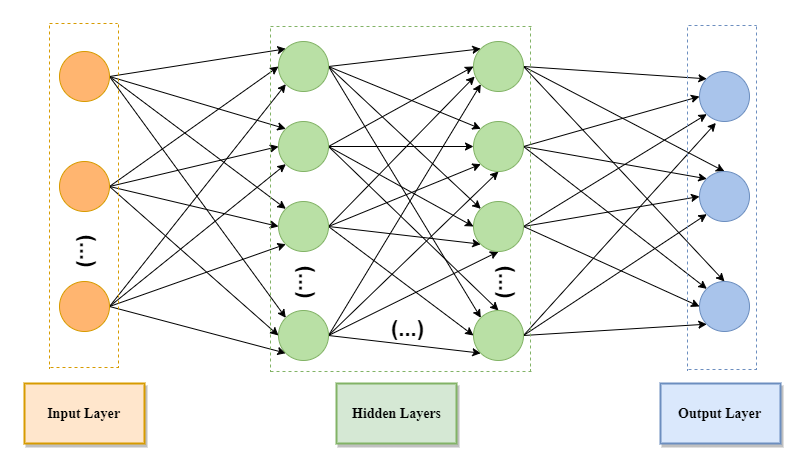
\includegraphics[width=0.8\textwidth]{Figures/mlp.png}
    \caption{Deep Neural Network Structure}
    \label{MLP}
\end{figure} 

Each input to a neuron contributes differently to the output. The share is
dependent on the weight value. These are obtained by training the network
through various techniques, one of which is called Deep Supervised
Learning~\cite{deeplearning} . For a certain input, there is an expected output
and the real output of the NN. Then the loss function (the difference) is
calculated and the weight values are iteratively modified for improving the
outputs of the NN.

A Deep Neural Network (DNN) is a Neural Network that uses this approach for
learning. It has multiple hidden layers and it can model complex non-linear
relationships. If the activation function is non polynomial, it satisfies the
Universal approximation problem~\cite{approximation:problem}.

One of the limitations of traditional NNs is the complexity of layer
interconnections. Using as example the hand digit recognition problem and MNIST
data set, composed of 28x28 grayscaled images~\cite{mnist:digits}, in a
traditional fully connected NN, a neuron from the second layer would have 28x28
weights. That is 3.136 kiloBytes per neuron of weight values while using 32-bit
floating-point numbers (FP32). When building a more complex network for image
recognition, the computationally complexity grows quadratically with the number
of neuros per layer.

%One propriety of CNN's is the shift invariance due to the use of 2D image convolution with filters and that makes them specifically
%good for Image and video recognition.

\section{Convolutional Neural Networks}
\label{section:subcnn}

Convolutional Neural Networks (CNN) are a class of DNNs used in Image and Video
recognition due to their shift invariance characteristic. They were first
proposed in the 1980s but it was not until 2012 with AlexNet~\cite{alexnet} that
CNNs really took off. Fundamentally, CNNs are a regularized version of
Multilayer Perceptrons (MLP). These networks fix the complexity issue discussed
as each neuron is only connected to a few neurons of the previous layer.
 

 \begin{figure}[!htbp]
    \centering
    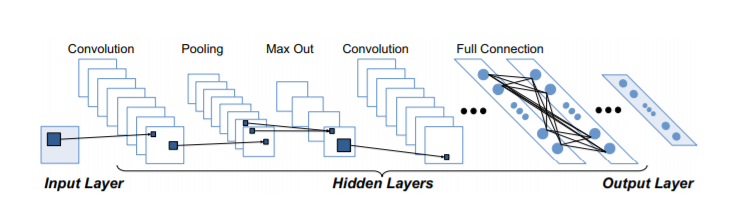
\includegraphics[width=1\textwidth]{Figures/convolutionlayer.png}
    \caption{CNN architecture example, taken from~\cite{cgracnn}}
    \label{CNNl}
\end{figure} 

 \subsection{Architecture Overview}
 \label{section:Aoverview}

 %There's several types of layers used in these networks to achieve the desired result.

 \subsubsection{Convolutional Layer}
\label{section:convlayer}

In a typical CNN not all layers are convolutional,but the convolutional layers
are the most compute intensive ones. CNNs take input images with 3 dimensions
(width, height and color space); for the following convolutional layers 3D
arrays are used (width, height and number of channels). For the earlier example
of the MNIST data set, the input would have dimensions 28x28x1 as it is a 2D
image in grayscale.

To compute a neuron in the next layer we get the convolution in
equation~\ref{equation:convolution} and image representation in figure \ref{Cl},
where $x_{j}^{l+1}$ is the output, $\delta$ is the activation function, which
depends on the architecture, $x_{i}^{l}$ is the input of the convolution layer,
$k_{ij}^{l+1}$ is the kernel of said layer which is obtained by training the
network and $b_{j}^{l+1}$ is the bias.
\begin{equation} \label{equation:convolution}
   %\resizebox{.5 \textwidth}{!} 
    %%
\end{equation}

Thus an output neuron depends only on a small region of the input which is
called the local receptive field.

\begin{figure}[!htbp]
    \centering
    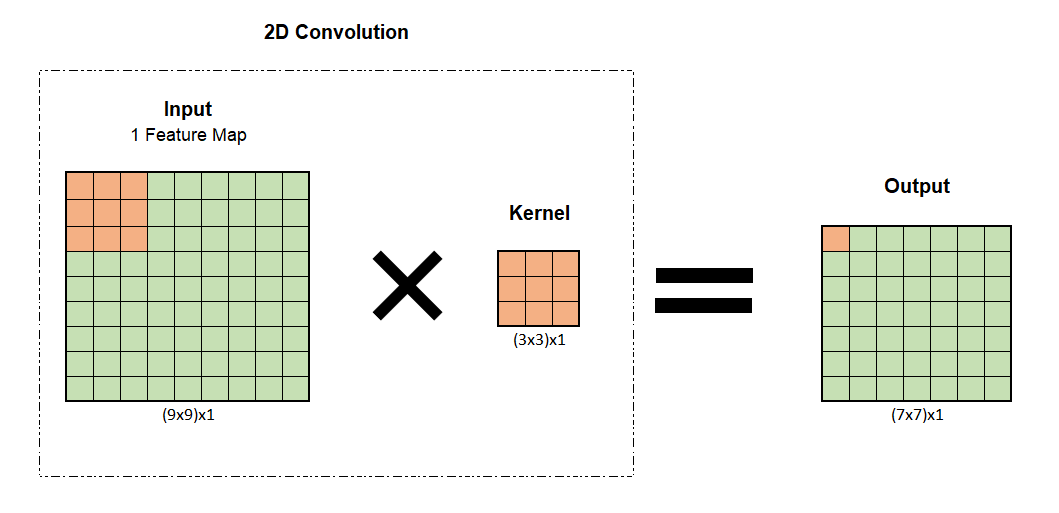
\includegraphics[width=1\textwidth]{Figures/conv.png}
    \caption{2D convolution with stride = 1 and without zero padding}
    \label{Cl}
\end{figure} 

The output's dimensions depend on several parameters of the convolution such as
zero-padding and stride. The Former means to add zeros around the edges of the
input matrix. The latter means the step used for the convolution, if the value
is e.g 2, it will skip a pixel each iteration of the convolution.  The equation
in~\ref{equation:padding} can be used to calculate the output size. Where $n$ is
the width/height of the input of layer $l$, $ b$ is the width/height of the
kernel, $p$ is zero-padding while $s$ is the stride.

\begin{equation} \label{equation:padding}
     n^{l+1} = \frac{n^{l}- b^{l}+2 \times p}{s}
\end{equation}

The number of channels of the output is equal to the number of filters in the
convolutional layer.


%Then a 3D convolution is performed with the kernel changing from layer to layer

\subsubsection{Pooling Layer}

The MaxPool or AvgPool are layers used in Convolutional Neural Networks to
downsampling the feature maps to make the output maps less sensitive to the
location of the features.

Maximum Pooling or MaxPool, like it is suggested in its name groups $ n * n $
points and outputs the pixel with highest value.  The output will have its size
lowered by $ n $ times.  The Average Pooling or AvgPool, instead takes all of
the input points and calculates the average. Downsampling can also be achieved
by using convolutions with stride 2 and padding equal to 1.  Upsample layers can
be also used that turn each pixel into $ n^{2} $, where n is the amount of times
the output will be bigger than the input.

\begin{figure}[!htbp]
    \centering
    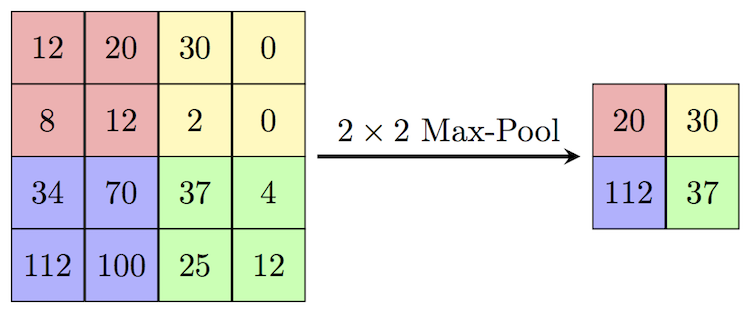
\includegraphics[width=0.5\textwidth]{Figures/maxpool.png}
    \caption{Simple example of a maxpool layer, taken from~\cite{maxpoolimg}}
    \label{figure:maxpool}
\end{figure} 
 

\subsubsection{Fully Connected Layer}

The fully Connected Layer is mostly used for classification in the final layers
of the Neural Network. It associates the feature map to the respective labels.
It takes the 3D vector and outputs a single vector thus it is also known as
flatten.  The equation in~\ref{equation:connected} describes the operation. Here
$w_{ji}^{l+1}$ are the weights associated with a specific input for each output
pixel.



\begin{equation} \label{equation:connected}
    %\resizebox{.5 \textwidth}{!} 
     %%
 \end{equation}
 

\subsubsection{Route $\&$ Shortcut Layer}

The Shortcut layer or skip connection was first introduced in
Resnet~\cite{resnet}.  It allows to connect the previous layer to another to
allow the flow of information across layers.  The Route layer, used in
Yolov3~\cite{yolov3} ,concatenates 2 layers in depth (channel) or skips the
layer forward. This is used after the detection layer in Yolov3 to extract other
features.

\subsubsection{Dropout Layer}

This type of layer was conceived to avoid overfitting~\cite{Dropout} by dropping
the neurons with probability below the threshold. In
figure~\ref{figure:Dropout}, there is a graphical representation.
\begin{figure}[!htbp]
    \centering
    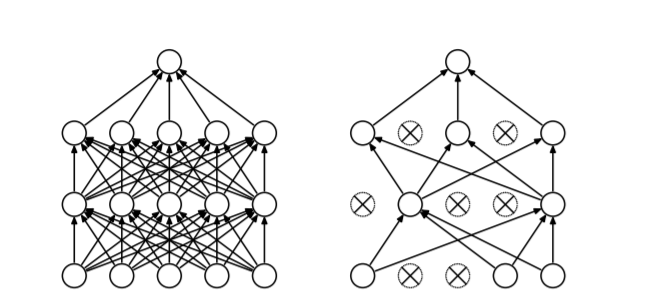
\includegraphics[width=0.6\textwidth]{Figures/dropout.png}
    \caption{Dropout if applied to all layers, adapted from~\cite{Dropout}}
    \label{figure:Dropout}
\end{figure} 

\subsubsection{Activation Functions}

Activation Functions (AF) are functions used in each layer of a Neural Network
to compute the weighted sum of input and biases, which is used to give a value
to a neuron.Non-linear AFs are used to transform linear inputs to non-linear
outputs.  While training Deep Neural Networks, vanishing and exploding
gradients.  are common issues, in other words, after successive multiplications
of the loss gradient, the values tend to tend to 0 or infinity and thus the
gradient disappears.  AFs help mitigate this issue by keeping the gradient in
specific limits. The most popular activation functions can be found in
table~\ref{table:AF}.

\begin{table}[]
    \centering
    \resizebox{.6\textwidth}{!}{%}
    \begin{tabular}{ll}
    \hline
    \textbf{Activation Functions} & \textbf{Computation Equation} \\ \hline \hline
    Sigmoid                       &  $\displaystyle f(x)=\frac{1}{1+ e^{-x}}$                             \\ \hline
    Tanh                          &  $\displaystyle f(x)=\frac{e^{x}-e^{-x}}{e^{x}+e^{-x}}$                            \\ \hline
    Softmax                       &  $\displaystyle f(x_{i})=\frac{x_{i}}{\sum_{j}e^{x_{j}}}$                             \\ \hline
    ReLU                          &    $ f(x)=\begin{matrix}
        x & if & x\geq 0  \\ 
        0 & if & x< 0 
    \end{matrix} $                           \\ \hline
    LReLU                         &  $f(x)= \begin{matrix}
        x & if & x > 0  \\ 
        \alpha x & if & x \leq 0 
    \end{matrix} $                        \\ \hline
    ELU                           &             $ f(x)=\begin{matrix}
        x & if & x> 0  \\ 
        \alpha e^{x} - 1 & if & x\leq 0 
    \end{matrix} $                 \\ \hline
    \end{tabular}%
    }
    \caption{Popular Activation functions}
    \label{table:AF}
\end{table}


%image of activation functions?

 \section{Frameworks for Neural Networks}
 \label{section:darknet}

To run a Neural Network model there are several popular frameworks like
Tensorflow, PyTorch, Caffe and Darknet.  Their purpose is to offer abstraction
to software developers that want to run these networks. They also offer
programming for different platforms like nVidia GPUs by using the CUDA API.

\subsection{Darknet}

Darknet~\cite{darknet} is an open source neural network framework written in C
and CUDA.It is used as the backbone for Yolov3~\cite{yolov3} and supports
several different network configurations such as AlexNet and Resnet.  It
utilizes a network configuration file (.cfg) and a weights file (.weights) as
input for inference.

\lstinputlisting[label=cfg,language=Python,frame=single,breaklines=true,firstline=13,lastline=19,caption=cfg
  code for a Convolutional Layer used in
  Yolov3~\cite{yolov3}]{./Code/yolov3.cfg}

In listing \ref{cfg}, there is a snippet of the file featuring a convolution
layer with 32 kernels of size 3x3. It has stride of 1 and zero padding of 1,
meaning the output size will be equal to the input. The input size can be
calculated by analyzing the previous layers and the network parameters. The
network parameters in \ref{net} includes data to be used for training while only
the first three parameters are needed for inference.

\lstinputlisting[label=net,language=Python,frame=single,breaklines=true,firstline=1,lastline=11,caption=cfg
  code for the network parameters]{./Code/yolov3.cfg}


\subsection{Caffe}

Convolutional Architecture for Fast Feature Embedding (Caffe)~\cite{caffe} is
also an Open source framework written in C++ with interface for Python.  Caffe
exports a neural network by serializing it using the Google Protocol Buffers
(ProtoBuf) serialization library. Each network has 2 prototxt files:
\begin{itemize}
    \item deploy.prototxt- File that describes the structure of the network that
      can be deployed for inference.
    \item train\_val.prototxt- File that includes structure for training.  it
      includes the extra layers used to aid the training and validation process.
\end{itemize}

The interface for python helps generate these files. For inference only the
deploy file matters.

\lstinputlisting[label=caffe,language=Python,frame=single,breaklines=true,firstline=1,lastline=26,caption=prototxt
  file for the input data and the first convolution layer of
  AlexNet~\cite{alexnet}]{./Code/caffe.prototxt}

\section{Deep Versat}
\label{sector:DeepVersat}

\quad Versat is a Coarse Grained Reconfigurable Array (CGRA) Architecture. CGRAs are in-between Field Programmable Gate Arrays (FPGA)
 and general purpose processors (GPP).
The former is fully reconfigurable and the highest performance for a workload can be achieved as the Architecture is tailored to the workload.
GPPs on the other hand, are not reconfigurable and thus slower but are more generic and can process different workloads.
While FPGAs have granularity at the gate level, CGRAs have granularity at the functional unit level. They are configurable at run-time and the datapath can be
changed in-between runs.   

In this chapter, the base Versat Architecture will be explained and then the Deep Versat Architecture
 and its improvements.

\subsection{Versat Architecture}

\quad The Versat Architecture~\cite{sousa:compiler,sousa:controller,sousa:FFT,sousa:versat2016} 
is depicted in Figure~\ref{figure:oldversat}. It is composed of the following modules: DMA, Controller, Program Memory, Control File Registry, Data Engine and Configuration module.
The Controller accesses the modules through the control bus. The code made in assembly or C is loaded into the program Memory (RAM) where the user
can write to the configuration module for the Versat runs. Between runs of the Data Engine,
 the Controller can start doing the next run configuration and calculations.


\begin{figure}[!htbp]
    \centering
    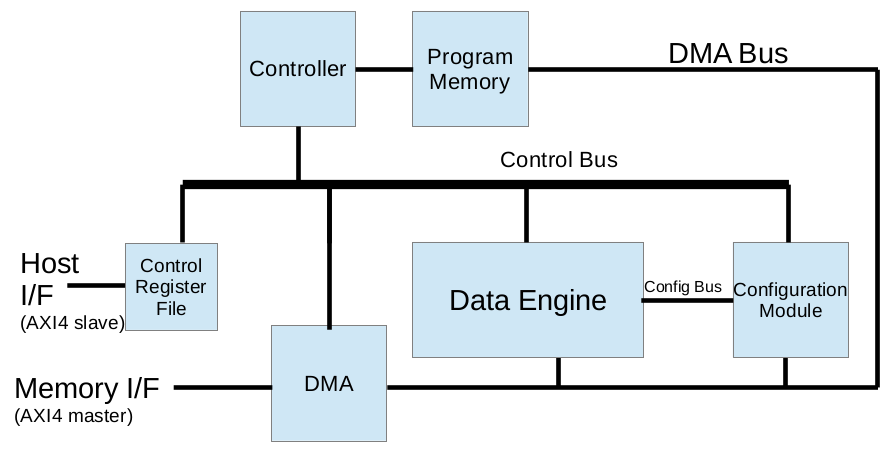
\includegraphics[width=0.8\textwidth]{Figures/top.png}
    \caption{Versat Topology, taken from~\cite{sousa:controller}}
    \label{figure:oldversat}
\end{figure} 

\subsubsection{Data Engine}
\quad The Data Engine which is represented in Figure~\ref{figure:DE} carries out the computation needed on the data arrays. It is a 32-bit architecture with up to 11 Functional Units (FU):
 Arithmetic and Logic Unit(ALU), stripped down ALU (ALU-Lite),
 Multiplier and Accumulator (MAC) and Barrel Shifter.
 Depending on the project and calculations, a new type of FU or the existing ones can be altered to support the algorithm.
 The DE has a full mesh topology, which means that each FU can be the output to another, which leads to a decrease in operating frequency.

 Each Input of a Functional Unit has a Mux with 19 entries, 8 of which are from the memories (2 from each Mem out of 4 total units) and the rest from the Functional Units (11).

 \begin{figure}[!htbp]
    \centering
    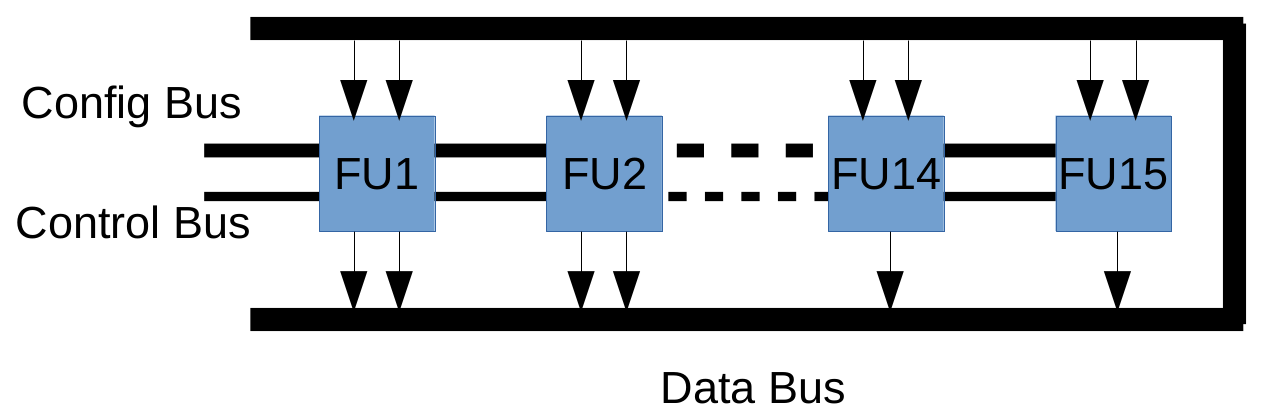
\includegraphics[width=1\textwidth]{Figures/de.png}
    \caption{Versat Data Engine Topology, taken from~\cite{sousa:FFT}}
    \label{figure:DE}
\end{figure} 

 The 4 Memories are dual port and for the input of both ports, 
 there is an Address Generation Unit (AGU) that is able to 
 reproduce two nested loops of memory indexes.
 The AGUs control which MEM data is the input of the FUs and where
 to store the results of the operation. Also, the AGUs support delayed start to line up timings
due to latencies. The memory module is represented in Fig~\ref{figure:FU}.

\begin{figure}[!htbp]
    \centering
    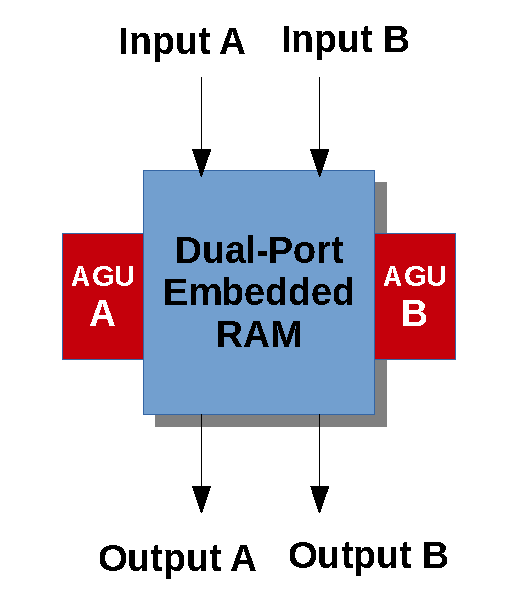
\includegraphics[width=0.5\textwidth]{Figures/fu2.pdf}
    \caption{Versat Memory Unit with one AGU per port, taken from~\cite{lopes:Versat}}
    \label{figure:FU}
\end{figure} 


\newpage
\subsection{Configuration Module}
\quad Versat has several configuration spaces devised for each Functional Unit,
with each space having multiple fields to define the operation of the Functional unit (e.g which op for the ALU).
These are accessed before the run by the controller to define the datapath.

\begin{figure}[!htbp]
    \centering
    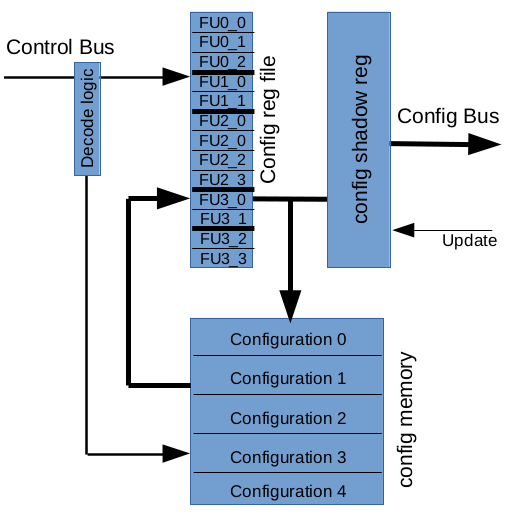
\includegraphics[width=0.6\textwidth]{Figures/conf.png}
    \caption{Configuration Module,taken from~\cite{sousa:controller}}
    \label{figure:conf}
\end{figure} 

The Configuration Module (CM), depicted in figure \ref{figure:conf}, 
has three components: configuration memory, variable length configuration register file 
and configuration shadow register.
The latter holds the current configuration so the controller can change the values of the configuration file in-between runs.
The decode logic finds which component to write or read, if it's the registers, it ignores read operations.
Meanwhile, the configuration memory interprets both write and reads. When it receives a read,
it writes into the register configuration data, when it's a write, it stores the data instead.


\newpage
\subsection{Deep Versat Architecture}


\begin{figure}[!htb]
    \centering
    \includegraphics[width=0.7\textwidth]{Figures/deep-Versat.png}
    \caption{Deep Versat Architecture, taken from~\cite{valter:deepversat}}
    \label{figure:deepversatarch}
\end{figure} 

\quad The Deep Versat Architecture~\cite{valter:deepversat}
, in figure~\ref{figure:deepversatarch}, decouples the Data Engine (DE) from all control and as such, it can be used with any CPU. 
It can be paired with hard cores in
FPGA boards like the ZYNC board %cite here
with its A9 ARM dual-core CPUs or pair it with a soft core.

Its principle is to create the concept of a Versat Core: Configuration Module (CM) and its Functional Units (FU) connected with a control bus and a data bus.
Instead of writing to memory, there is the option to write for the next
Versat Core to create more complex and more complete Datapaths, to avoid
having to reconfigure the cores.

The number of Layers and FUs are reconfigurable pre-silicon with the only limitation
that each layer is identical. To program Deep Versat, an API is generated
from the Verilog .vh files. 




\newpage
\subsubsection{Deep Versat System}

\begin{figure}[!htbp]
    \centering
    \includegraphics[width=0.8\textwidth]{Figures/deep-Versat-top.png}
    \caption{Deep Versat System using a RISC-V RV32IMC soft core, taken from~\cite{valter:deepversat}}
    \label{figure:deepversattop}
\end{figure} 

\quad To make a complete system, a new controller is needed with a more robust toolchain.
In a recent dissertation~\cite{valter:deepversat}, the IOB-RV32 processor was used which uses the RISC-V Instruction Set (ISA) with 32-bit Integer base alongside Multiplication and Division extension and Compact Instruction extension.
 The core is derived from
the open-source PicoRV32 CPU~\cite{picorv}.
The IOB-RV32 uses its memory bus to access peripherals in which Deep Versat and the UART module are connected as such.
The control bus is used to access the configuration modules of Deep Versat. The data bus is used to read and write
a large amount of data into Deep Versat. The data flow bus is reserved for inter-Versat Core communication.

\begin{table}[!htbp]
    \centering
    \begin{tabular}{|ll|}
        \hline
        \textbf{Peripheral}     & \textbf{Memory address} \\ \hline
        UART module             & 12’h100xxxxx            \\ \hline
        Deep Versat control bus & 8’h11xxxxxx             \\ \hline
        Deep Versat data bus    & 8’h12xxxxxx             \\ \hline
        \end{tabular}
    \caption{Deep Versat Memory Map}
    \label{table:deepversat}
    \end{table}


The memory map to address the peripherals,
 including deep Versat, is in table \ref{table:deepversat}.
 Each Versat has 15 bits of address while the CPU addresses
 the peripherals with 32 bits, with 8 of those occupied to choose
 the peripheral in question. That leaves 9 bits to address several Versat Cores
 which brings the theoretical maximum Versat cores to 512. The IOB-RV32 is compatible with the
 GNU toolchain to offer better portability of code and alongside the C++ Versat API the difficulty
 to code for the System diminishes.
%%%%%%%%%%%%%%%%%%%%%%%%%%%%%%%%%%%%%%%%%%%%%%%%%%%%%%%%%%%%%%%%%%%%%%%%%
%                                                                      %
%     File: Thesis_Implementation.tex                                  %
%     Tex Master: Thesis.tex                                           %
%                                                                      %
%     Author: Andre C. Marta                                           %
%     Last modified :  2 Jul 2015                                      %
%                                                                      %
%%%%%%%%%%%%%%%%%%%%%%%%%%%%%%%%%%%%%%%%%%%%%%%%%%%%%%%%%%%%%%%%%%%%%%%%

\chapter{Implementation}
\label{chapter:implementation}

Insert your chapter material here...

%%%%%%%%%%%%%%%%%%%%%%%%%%%%%%%%%%%%%%%%%%%%%%%%%%%%%%%%%%%%%%%%%%%%%%%%
\section{Numerical Model}
\label{section:model}

Description of the numerical implementation of the models explained in Chapter~\ref{chapter:background}...


%%%%%%%%%%%%%%%%%%%%%%%%%%%%%%%%%%%%%%%%%%%%%%%%%%%%%%%%%%%%%%%%%%%%%%%%
\section{Verification and Validation}
\label{section:verification}

Basic test cases to compare the implemented model against other numerical tools (verification) and experimental data (validation)...

 % file "Thesis_Implementation.tex"
\chapter{CNN Compiling and Computation}
\label{chapter:CNNVersat}

This chapter presents an overview of toolflows that map convolutional neural
networks into FPGA using the frameworks presented in
Section~\ref{section:darknet}. Next, the concepts for mapping CNNs
into CGRAs are introduced.

%PAPERS
%https://www.cv-foundation.org/openaccess/content_cvpr_workshops_2014/W17/html/Gokhale_A_240_G-opss_2014_CVPR_paper.html
%

\section{Toolflows for Mapping CNNs in FPGAs}
\label{section:toolflow}

Several software frameworks have been developed to accelerate development and
execution of CNNs. The neural networks frameworks discussed in
section~\ref{section:darknet} provide high level APIs together with high
performance execution on multi-core CPUs, GPUs, Digital Signal Processors (DSPs)
and Neural Processing Units (NPUs)~\cite{smartphones}. FPGAs provide an
alternative to these architectures as they provide high-performance while also
being low-power. FPGAs can meet several requirements like throughput and latency
in diversity of applications. Thus, several toolflows that map CNN descriptions
into hardware in order to perform inference have been created. In
table~\ref{table:toolflow}, a list of notable ones is presented.

\begin{table}[!htpb]
    \centering
    \begin{tabular}{lll}
    \hline
    \textbf{Toolflow Name} & \textbf{Interface}       & \textbf{Year}  \\ \hline
    fpgaConvNet            & Caffe \& Torch           & May 2016       \\
    DeepBurning            & Caffe                    & June 2016      \\
    Angel-Eye              & Caffe                    & July 2016      \\
    ALAMO                  & Caffe                    & August 2016    \\
    Haddoc2                & Caffe                    & September 2016 \\
    DNNWeaver              & Caffe                    & October 2016   \\
    Caffeine               & Caffe                    & November 2016  \\
    AutoCodeGen            & Proprietary Input Format & December 2016  \\
    Finn                   & Theano                   & February 2017  \\
    FP-DNN                 & Tensorflow               & May 2017       \\
    Snowflake              & Torch                    & May 2017       \\
    SysArrayAccel          & C                        & June 2017      \\
    FFTCodeGen             & Proprietary Input Format & December 2017  \\ \hline
    \end{tabular}
    \label{table:toolflow}
    \caption{CNN to FPGA Toolflows, adapted from~\cite{misc:cnntofpga}}
\end{table}


\subsection{Supported Neural Network Models}

These toolflows support the most common layers in CNNs, which are discussed in
chapter~\ref{chapter:cnn}. The acceleration target changes depending on the
toolflow.  For example, the fpgaConvNet~\cite{fpgaconvnet} toolflow focuses more
on feature extraction while offering non accelerated support for fully connected
layers by
%FIX
casting them as Convolutional Layers with 1x1 kernels. 

\subsection{Architecture \& Portability}

\begin{figure}[!htbp]
    \centering
    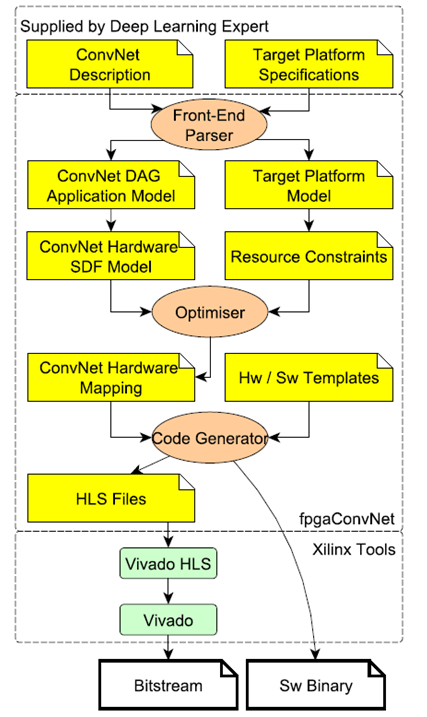
\includegraphics[width=0.5\textwidth]{Figures/fpgaconvnet.png}
    \caption{fpgaConvNet Architecture. Taken from~\cite{fpgaconvnet}}
    \label{figure:fpgaconvnet}
\end{figure}

As shown in figure~\ref{figure:fpgaconvnet}, the fpgaConvNet architecture
consists of a Front-End Parser that reads a (ConvNet) description of the network
and a description of the target platform and produces, on the one hand a
Directed Acyclic Graph (DAG), which is then converted to a Synchronous Data Flow
(SDF) hardware model, and on the other hand, a model of the target platform from
which resource constraints are derived. The hardware model thus obtained goes
into an Optimiser procedure, which produces a hardware mapping. Using hardware
and software templates, a Code Generator procedure, generates both the High
Level Synthesis (HLS) input files and the software binaries that will run on the
control CPU embedded in the FPGA. The HLS files go into the Xilinx (FPGA
manufacturer) tools so that the configuration bitstream of the FPGA is produced.

\newpage
\section{CNN Auto Tuning Framework}
\label{section:autotuning}
 % add new .tex files for new chapters
\cleardoublepage



%\chapter{Proposed Work and Planning}
\label{chapter:PWP}

The proposed work for the dissertation consists in the development of an
automatic compiler of DNN description into Deep Versat / IOB-RV32 C++ code. The
purpose of this work is to be able to run any state of the art CNN on the Deep
Versat system with no effort on the user side, allowing the design and
architectural exploration.

For the proof of concept stage, Darknet and Caffe will be the frameworks chosen
to be supported by the compiler. Deep Versat can customized with the number of
layers, numbers of each FU type and other options. Hence, the compiler must be
able to take the configurations into account when producing computational
datapaths for Deep Versat.

\section{Flowchart}

\begin{figure}[!htb]
    \centering
    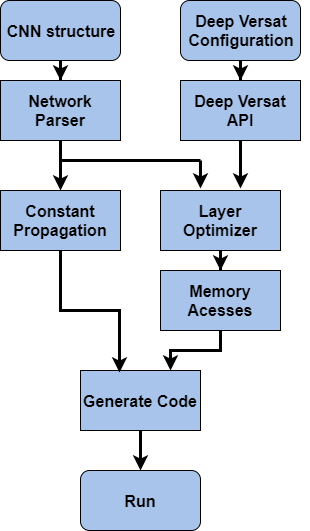
\includegraphics[width=0.5\textwidth]{Figures/flowchart.png}
    \caption{Flowchart of the software architecture}
    \label{figure:flowchart}
\end{figure}



Figure~\ref{figure:flowchart} presents the flowchart of the system to be developed. The steps
of the algorithm are explained in the next paragraphs.

%FIX Aproveitas o que está em bx para alguma box fo do fluxo grama ?
To build a CNN model for Versat, a parser from Configuration file to layer is needed. For darknet~\cite{darknet},
 the parser can be re-used.
For Caffe, a new one would need to be built so the output of the parser is equal to other frameworks for the same CNN network.
The objective to be accomplished is to support all Caffe possible layers and Darknet's layers.
After parsing the network, constant propagation is taken care of. That means,
%After parsing, the Versat dataflow and runs for each type of layer will be defined depending on current silicon set up of the CGRA. Then,
%the C code with the Versat runs will be written.

%FIX Aproveitas para alguma box fo do fluxograma ?
Some of the activation functions discussed in chapter \ref{chapter:cnn}
will have to be processed in software on the core unless custom Functional Units
are made for each function. Convolutional,Fully Connected,Shortcut and Route
layers can be implemented on Deep Versat without any FU changes. How much it
will be accelerated is based on number of cores and MACs available. Pooling
needs adaptation in Hardware to run them, if not implemented, run on the RISC-V
core.

\section{Workplan}

In fig~\ref{figure:gant}, a GANT chart with the proposed schedule for the
planned work is presented. Further explanations on each task will follow in the
next paragraphs.

\begin{figure}[!htbp]
    %\centering
    \includegraphics[width=1\textwidth]{Figures/gant2.png}
    \caption{GANT chart of Proposed Work}
    \label{figure:gant}
\end{figure}





 % add new .tex files for new chapters
%\cleardoublepage

% YoloLITE
\chapter{Darknet Lite}
\label{chapter:Darknet}

As mentioned in Section \ref{chapter:DeepVersat}, the Deep Versat system includes a RISC-V CPU to take out generic
code and to write the configuration runs into Versat's memories. This means the first step into implemetning software
that can run any convolutional neural network on this system, it must first run on the CPU then we off load Fixed Functions 
to Versat such as the convolutional layers, maxpool etc.

\section{Porting Darknet to an embedded CPU}

As mentioned in Section \ref{section:darknet} is a framework for Neural Networks on C++ that uses dynamic memory 
and GPU acceleration option to get faster outputs.
Also the use of floats is also prohibited in the embedded code
as the RISC-V CPU only supports the extentions IM. I for Integer and M for multiplication.
It also has a lot of features that are not needed in this work, such as training the CNN.
By stripping the features of darknet we get a much simpler
code framework apropriately named darknet lite.

In the following figure, 
the data strucuture for a layer is showed. A CNN on darknet lite is just an array of layers in which each has an input, 
output and layer parameters. 
Usually the input is a past layer output or the image input.

\lstinputlisting[label=DarknetLiteStrut,language=C++,frame=single,breaklines=true,firstline=1,lastline=38,caption=Layer Struct
  Yolov3~\cite{yolov3}]{./Code/DarknetLiteStrut.h}

By Parsing the .cfg file, a configuration file is written in C with the layer array and static position of the data for each layer. 
Each Layer has it's definition in C to be ran by the embedded CPU but for the sake of this project, several layers can be
replaced by Functions that utilize Versat, the same way that the original Darknet framework had it's functions written for CPU or GPU usage.

In the following figure is an example of a CPU layer that computes the convolutional layer while using Fixed Point Logic.

\lstinputlisting[label=ConvolutionalLayerCPU,language=C++,frame=single,breaklines=true,firstline=54,lastline=85,caption=Convolutional Layer using only CPU and fixed memory]{./Code/convolutional_layer.c}


\section{Conversion of Caffe to CFG}



\section{Parsing CFG Files into the program} % add new .tex files for new chapters
\cleardoublepage

% DeepVersat Simulator
\chapter{DeepVersat Software Simulator}
\label{chapter:Simulator}

The increasing complexity of configurations in the Versat platform and the time-consuming and challenging nature of hardware simulation and debugging have highlighted the need for an efficient software simulator. 
The primary objective is to emulate the hardware behavior with enhanced efficiency compared to traditional hardware simulation methods. 
This is particularly crucial as hardware development cycles are significantly longer compared to software development. 
The simulator operates by executing clock iterations, ensuring consistent results at each clock cycle, similar to the hardware execution. 
Leveraging the advantages of the Coarse-Grained Reconfigurable Array (CGRA) architecture of Versat, the simulator allows for easy implementation of different functional unit configurations and significantly reduces the time required to assess performance for specific programs. 
This chapter delves into the software architecture, object relationships, and provides a detailed explanation of the methods employed to emulate Versat clock by clock.

% The only data the simulator can't output
% is FPGA resource usage the hardware configurations fit the FPGA that is going to be used and the clocks that 
% the hardware can run. But, the propagation time is predictable depending on the number of 
% functional units as the difference between times in different setups are 
% due to the multiplexers on the inputs of the FUs.



\section{Architecture and Object Relation}

The simulator comprises the Parent Class, Versat, which will be simulated. As each Versat instance is independent of the others, the simulations are also separate.
The Versat is made up of two CStage Arrays, one is the "live" while the other is the 
shadow registers, where the configurations are held before the simulator is run.
Each stage is comprised of instances of the FUs defined in the hardware configuration file, each of which is connected to the Databus.
As it happens in the hardware, functional units can access the database, which has the output 
of the current stage and the previous stages' output.
\clearpage

\begin{figure}[!htbp]
    \centering
    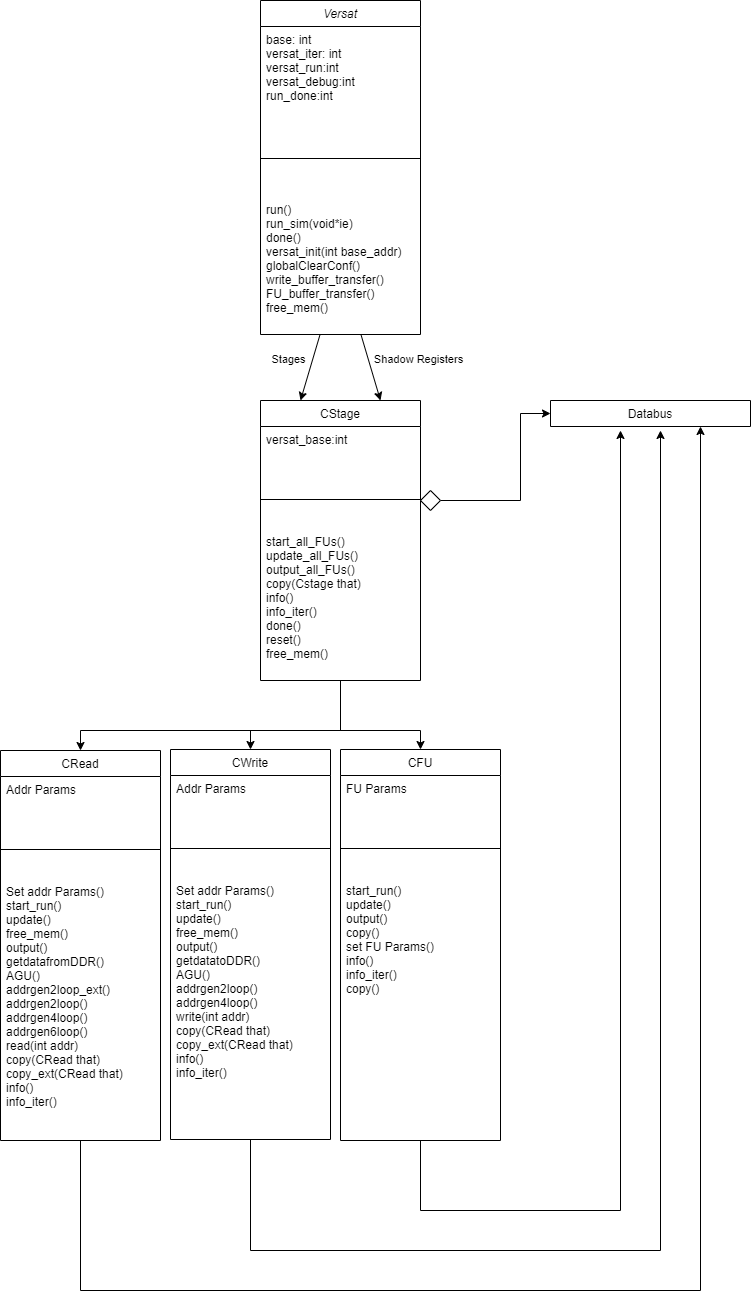
\includegraphics[width=0.8\textwidth]{Figures/VersatSimulatorDraw.drawio.png}
    \caption{Class Structure for the Versat Simulator}
    \label{figure:VersatSimulatorClass}
\end{figure} 


\subsection{Functional Units}

The following Table contains the functional units present in the simulator 
and is represented by 
"CFU" inFigure~\ref{figure:VersatSimulatorClass}. 
VI and VO represent CRead and CWrite 
classes respectively.



\begin{table}[!htbp]
    \centering
    \begin{tabular}{|ll|}
        \hline
        \textbf{Functional Unit}     & \textbf{Porpuse}  \\  \hline
        Read (VI) Mem Unit             & Reads from DDR and sends Data to databus            \\ \hline
        Write (VO) Mem Unit & Reads from databus and sends Data to DDR             \\ \hline
        MulAdd (MAC)    & Multiplication and Accumulate          \\ \hline
		Mul    & Multiplication     \\ \hline
		Alu    & Standard algorithmic and logic unit     \\ \hline
		AluLite    & Stripped down  algorithmic and logic unit     \\ \hline
		Barrel Shifter (BS) & Shifts to the right (division by 2) or to the left (multiplication by 2) \\ \hline
		Memory (Mem) & Sends/Receives data to/from the pipeline. Data is inserted through CPU communication   \\ \hline
        \end{tabular}
    \caption{Versat Simulator Functional Units}
    \label{table:versatsimfu}
    \end{table}

To add a new FU, it's as easy as creating a new class that CStage will use with
a run(), update(), output(), and copy() method. Of course, if it has variables needed to be defined
by the program, set param functions are also required. Using the simulator, hardware development
and program development can be parallelized to output a new program 
with more optimized performance.

In the next section, these methods will be explained in detail and 
their importance to the simulator.

\section{Simulation}

After the program that is running on the CPU finishes writing the configurations, it will call the run method of Versat.
InFigure\ref{figure:VersatSimulatorSequenceDiagram}, a sequence diagram is presented with the rundown
of a typical program that uses Versat Simulator.

\newpage
%Previously, a software API was made in a previous thesis~\cite{valter:deepversat}
%for Versat. To build on top of this several, software functions were added to make writing configurations to Versat
%easier.
\begin{figure}[!htbp]
    \centering
    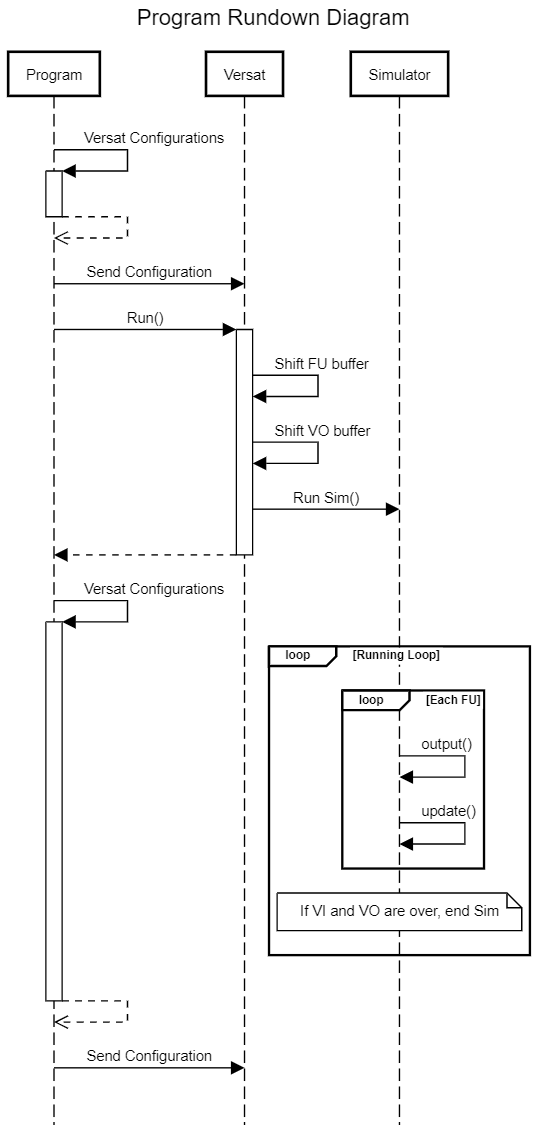
\includegraphics[width=0.7\textwidth]{Figures/versatsim.png}
    \caption{Sequence Diagram of a Program using Versat Simulator}
    \label{figure:VersatSimulatorSequenceDiagram}
\end{figure} 



\subsection{Run() Function}

In the software API for Embedded Versat, the run function would write to a shadow register,
which we can call "start", changing the value from zero to 1. 
Similarly, another register would
change the value to 0, which we can call "done". While this last register isn't turned to 1, 
Versat hasn't finished running with the 
previous configurations, so all that can be done is to write
configurations for future runs.

In the simulator, it works in a similar way to preserve compatibility 
as the goal is to have the same
programs run on software simulators and the FPGA.

\lstinputlisting[label=runfunctioncode,language=C++,frame=single,breaklines=true,firstline=222,lastline=245,caption= The Run function code]{./Code/Versat.cpp}

As we can see in the previous Listing, we reset the state variables of the simulator, then shift the VO and FU shadow registers.
This is done to simulate the pipeline delay in the FPGA. 
Because the data needs to come and go to the main memory (DDR),
One run cycle is used just for fetching data and writing data. 
Using a small example:
If a developer writes a configuration to do a 5x5 matrix multiplication, 
Versat will have to run three times.
Once to fetch data from memory, the second for the actual use of Versat 
and the final one is to get data onto memory.

In the simulator, this is done using the same class instances and 
copying the configuration values. On the hardware, it's several flip-flop registers in a row.
However, all these three stages can happen at once if you run multiple configurations in one program, e.g., running a CNN
through Versat will have at least one run per layer. 
So, if it has five layers, Versat will have to run 5+2 times. The last two times are done to
flush the Versat of any data.

After the shift, a new thread is created to run the simulator in parallel 
with the configurations,
having the same behavior as the hardware.

\subsection{Start() Method}

At the beginning of the configuration run, the method "start run" of 
all FUs and memories are started.
In this function, several functional units will have their state variables reset, such as VI, VO, and MAC FU.

\subsection{Databus}

The databus on Versat is a simple array that holds all the outputs of the functional units.
The array's data type (versat\_t) depends on the width of Versat, which is part of the configuration file.
Using higher width, e.g., 64 bits, is useful for the single instruction, multiple data (SIMD) 
applications but requires the functional units to be adapted.
For the purpose of this thesis, 16 bits and 32 bits are used depending 
on the neural network and how it is optimized.

When the Versat is instanced in the program, the functional units constructor will point
to the correct position of the databus as referenced in the following figure.

As mentioned inFigure\ref{figure:deepversatarch} from chapter \ref{chapter:Background}, section \ref{sector:DeepVersat}, 
each functional unit will be able to access the output from the functional units of the
current stage and previous. Software-wise, each stage will be pointing to a part of the databus.  

% INSERT FIGURE HERE


\subsection{Update() and Output() Method}


The update method's goal is to update the functional unit's value on the databus. 
Each functional unit has a pipeline delay to output or has a run delay configured, 
like the memories or MAC.

Meanwhile, the output method's goal is to, based on the inputs from the databus, calculate the result from
 the functional unit.

 For computing functional units such as the MAC or the ALU, this means reading from the databus for operands A and B
 and performing the selected operation. For the read memory (VI), it will output an address on the mem
 and performs a read operation. For the write memory, it will output an address and performs a write operation.

 In the Listing\ref{listing:fu}, the code of the Mul functional unit is used as an example.

 \newpage
 \lstinputlisting[label=listing:fu,language=C++,frame=single,breaklines=true,firstline=21,lastline=65,caption=Update and Output method of Mul]{./Code/mul.cpp}


\subsection{Copy() and Info() Method}

Finally, the last two functions of the simulator are copy() and info(). The former primary purpose is to copy the configuration parameters from one instance to another,
used mainly at the beginning of the run to simulate the shadow registers.
Meanwhile, the info method is a state printing function that outputs a string with the complete data of the current iteration,
this way, there will be an output file iteration by iteration to check the progress of the simulation, just like in a hardware simulator.

\lstinputlisting[label=listing:fu,language=C++,frame=single,breaklines=true,firstline=572,lastline=584,caption=Info output for the MAC functional unit]{./Code/versat_iter22.txt}
 % add new .tex files for new chapters
\cleardoublepage

% Automatic Convolution Configuration Writer
\chapter{Versat API 2.0}
\label{chapter:API}

The Versat API, developed in a previous thesis~\cite{valter:deepversat}, has the ability to conceal
the calls to the hardware to avoid changing the program when the hardware changes. 

This chapter will discuss the new functions that are part of the Versat API. The goal
is to make development for Versat just like writing regular code and to be easy to port code the same way
CUDA has done the same to run SIMD code on Nvidia GPUs.

\lstinputlisting[label=listing:versathpp,language=C++,frame=single,breaklines=true,firstline=17,lastline=40,caption=Sample Versat API implementation for the Hardware for Mem functional unit]{./Code/Versat.hpp}

\section{API Architecture}

Figure \ref{newAPI} presents a graphic representation of the new API. It has five apparent layers:

\begin{enumerate}
	\item Complex Mathematical API that is automatically optimized for the Versat Setup you chose. No dev work is required.
	\item Read/Write using VI and VO for simpler data setup. It also includes easier FU functions to set up workloads.
	\item Read/Write configurations for inside Versat Data (Int) or DDR to/from VI/VO (Ext).
	\item Versat API 1.0 where each configuration variable needs to be set up individually
	\item No API. Hardware registers where the values are used inside Versat. 
  \end{enumerate}


\begin{figure}[!htbp]
    \centering
    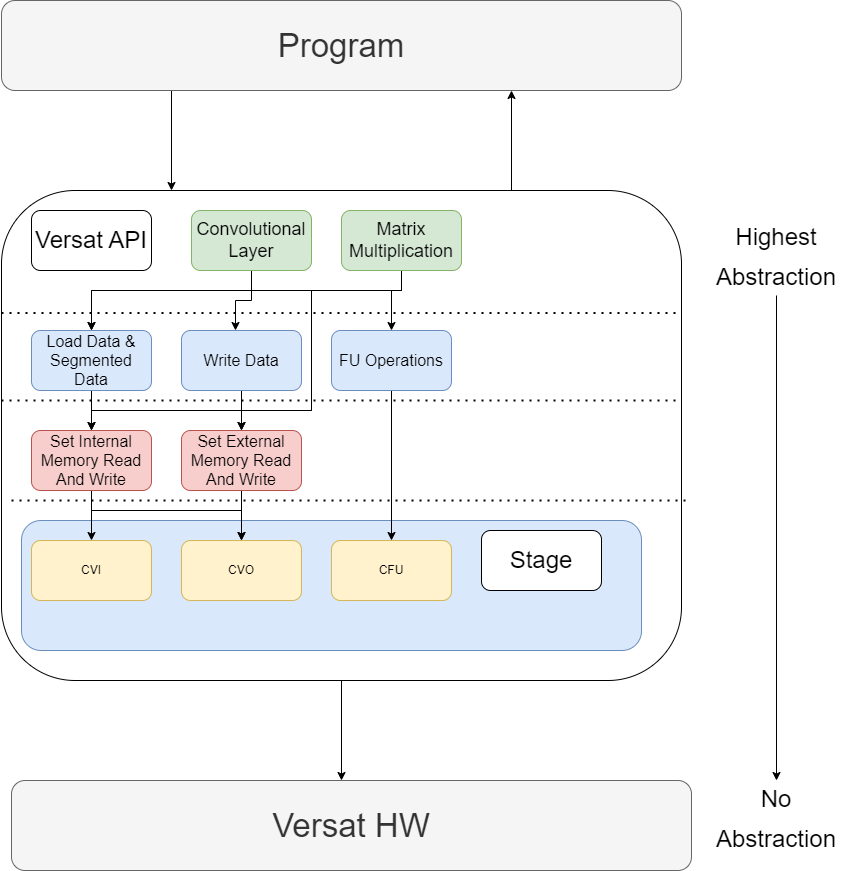
\includegraphics[width=0.7\textwidth]{Figures/VersatMemory.drawio.png}
    \caption{Graphic representation of the new Versat API and its connections}
    \label{newAPI}
\end{figure} 


\section{Memory Operations API}

When utilizing the VI instead of a MEM, the data transfer happens between the functional unit and direct memory access. At the same time,
on the mem, the CPU writes directly to Versat, wasting CPU cycles. For the API, this means going from a straightforward read method
to more configuration methods to set up the read operation from DDR. The same happens to Write operations. To address this, seven functions were created in two levels of abstraction:
load\_data(),load\_segmented\_data(),write\_data() that use a lower level functions: set\_IntMem\_Write(),set\_ExtMem\_Write(),set\_IntMem\_Read() and set\_ExtMem\_Read().
The function of the higher abstraction memory functions is to abstract the parameters of the AGU. In the following Listing, we have one of the implementations
as an example.

\lstinputlisting[label=listing:loadsegdata,language=C++,frame=single,breaklines=true,firstline=366,lastline=376,caption=Load Segmented Data code]{./Code/versat_configurations.cpp}


Although this means having to write code with the AGUs in mind
and how they function. To avoid it, a new class was created, shown in Listing\ref*{listing:accumulator},
to abstract how the AGU counts loops and approximate 
the code to simple C++ code that runs on a CPU.

\lstinputlisting[label=listing:accumulator,language=C++,frame=single,breaklines=true,firstline=72,lastline=110,caption=Accumulator Class code]{./Code/versatnew.hpp}

To transform from AGU parameters to for loop, it depends on the number of loops pretended to be done. VI AGU is three  cascade Accumulators
and as such, the increment on the second and third accumulators needs to be adjusted, as shown below.

\lstinputlisting[label=listing:intmemread,language=C++,frame=single,breaklines=true,firstline=77,lastline=86,caption=AGU parameters to Simple forloop parameters transform]{./Code/versat_configurations.cpp}

\section{Matrix Multiplication and Dot Product}

As part of the new API, a matrix multiplication function was added. The code is presented in Listing\ref{listing:matrixmult}. First, two Accumulator class variables are initialized.
Afterward, using the two arrays address in DDR, the AGU configurations of the VIs to read from the main memory are set, then the AGU configurations of VI for the data handling inside the Data Engine.
Finally, the function will write the MAC configuration and the store AGU configurations. This last step is optional as the result of this matrix multiplication can be used in the same run
to make other operations, e.g., adding a bias using one of the ALUs to the results.

\lstinputlisting[label=listing:matrixmult,language=C++,frame=single,breaklines=true,firstline=167,lastline=215,caption=Matrix Multiplication Configurations]{./Code/versat_configurations.cpp}

The Dot product function is very similar. The configurations are identical for transferring data from the main memory to the VIs. In the inside loops of the VIs, instead of three  loops, we only need to use 
1.

\section{Generic Convolution}

As explained in chapter \ref*{chapter:Background}, convolutional neural networks are a type of neural net  
used mostly in image and object recognition using convolutional layers. To run a convolutional layer on Versat with
optimized performance, the configurations must be written with regard to several parameters:

\begin{enumerate}
	\item Memory Sizes used in VI and VO. The amount of data that can be stored at once. It determines the number of outputs done per run.
	\item Functional Units used in the Data Engine. Here it's about the lowest common denominator, i.e., the bottleneck in the Data Engine determines the number of outputs done simultaneously.
  \end{enumerate}
 
This function has a total of 20 variables calculated at the start before the Versat configurations are written. The most important
variables are the following:

\begin{itemize}
	\item output height (h) and width (w) of the resulting matrix from the convolution.
	\item Number of outputs done simultaneously, also known as pipeline width (nOutputs). This value is pre-compiled as it depends on only Versat Configurations.
	\item Number of outputs that can be done per VI (y) in a single run and its variations. Outputs total (y\textsubscript{2}), Output Lines per VI (y\textsubscript{3}) Output Lines total (y\textsubscript{4}).
The value of y4 and y2 decide the different configuration scenarios.
	\item Resource Allocation Variables
which are explained in subsection \ref*{ConvolutionScenarios}
	\item Address Variables
	\item AGU Configuration Variables
  \end{itemize}

The algorithm's hard part is allocating the data in the most efficient way possible and creating the AGU configurations
for the VIs and VOs. For this algorithm, the CGRA will act like a GPU pipeline where several "threads" will exist
that will output one point every k\textsuperscript{2} cycles, where k is the kernel size used in the convolution.

\begin{figure}[!htbp]
    \centering
    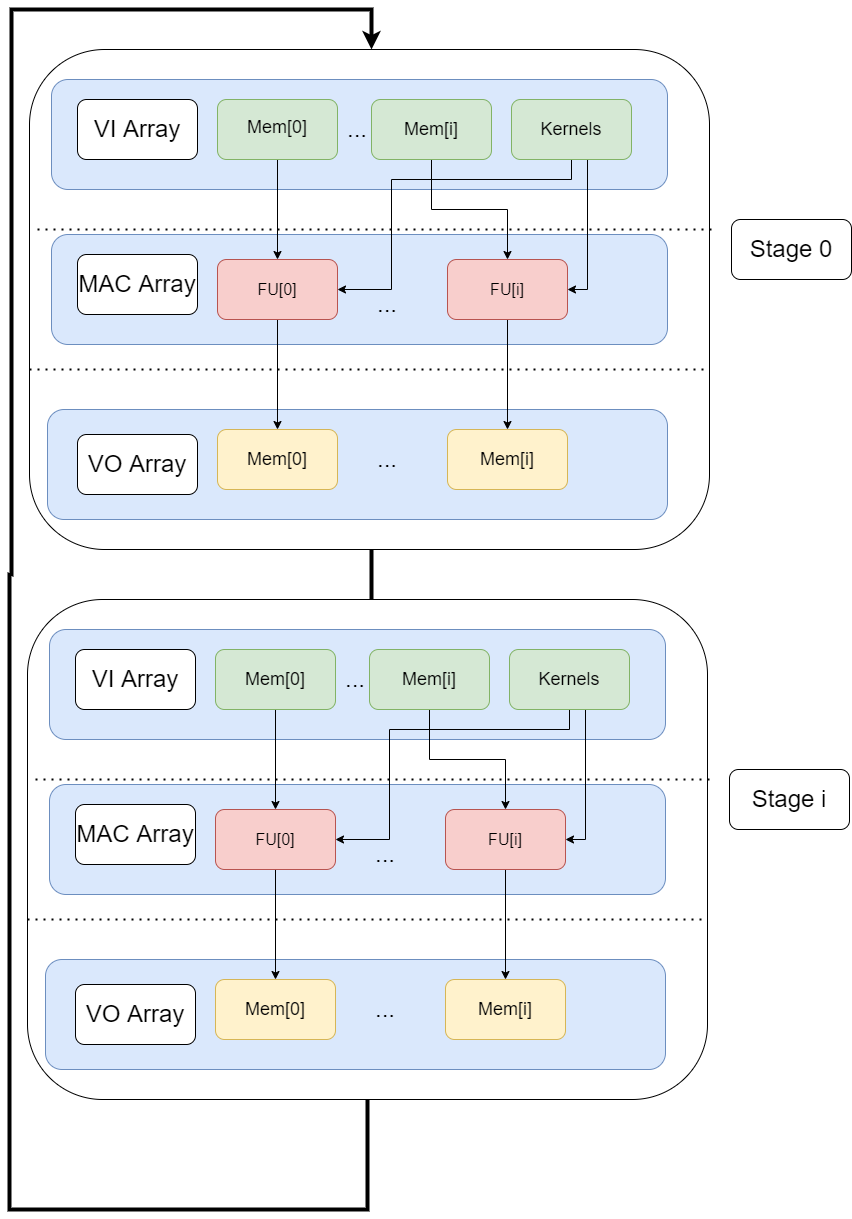
\includegraphics[width=0.7\textwidth]{Figures/Convolution.drawio.png}
    \caption{Versat Configuration goal in Graphical form}
    \label{VersatConfiguration}
\end{figure}

\subsection{Loading Data}

Usually, when doing a convolution in CPU, the frameworks transform the convolution to a matrix multiplication by creating a new matrix that will multiply with a
kernel vector. It's done this way as matrix multiply is a heavily optimized operation and can take advantage of a CPU's SIMD units or even call the GPU APIs
and offset the workload there. On Versat, this is not needed to calculate one output. We will need only enough space in mem to hold
k\textsuperscript{2}*ch where ch is the input channel. And as such, it means 9216 bytes per VI, at least for YoloV3 CNN when using 16-bit operands.

To load the data onto the mems in Versat, we will load segmented data. That is, for each mem, we will load the data
needed to do y iterations or y\textsubscript{3} iterations, depending on which convolution scenario it is.
The more inputs are transferred to a VI mem, the more efficient it is, as data doesn't need to be replicated as much between the instances,
i.e., for the first output, there's a need for k\textsuperscript{2}*ch inputs, but for other sequential outputs, if the stride is one, only k*ch more inputs are needed. But, of course, this is only true if the stride is lower than the kernel size.

This takes the form of the code in one line, thus the importance of the previously written functions.

\lstinputlisting[label=listing:memread,language=C++,frame=single,breaklines=true,firstline=446,lastline=446,caption=Load Input Matrix into VIs]{./Code/versat_configurations.cpp}

Where the variable "size per channel" can be calculated with the following formula:

\[ size=w*(k+stride*(iter-1)) \]

Where w is the width of the input matrix, k is the kernel size, and iter is the number of iterations that this mem will run.

\subsection{Convolution Scenarios}
\label{ConvolutionScenarios}

When writing the configurations of the convolution runs, the software needs to consider several cases.
As explained in the previous subsection, the data that the VIs can handle and the number of datapaths that the data can have influenced
the convolution scenarios. Four were implemented for this function and presented in Figure \ref{ConvScenarioss}.

\begin{figure}[!htbp]
    \centering
    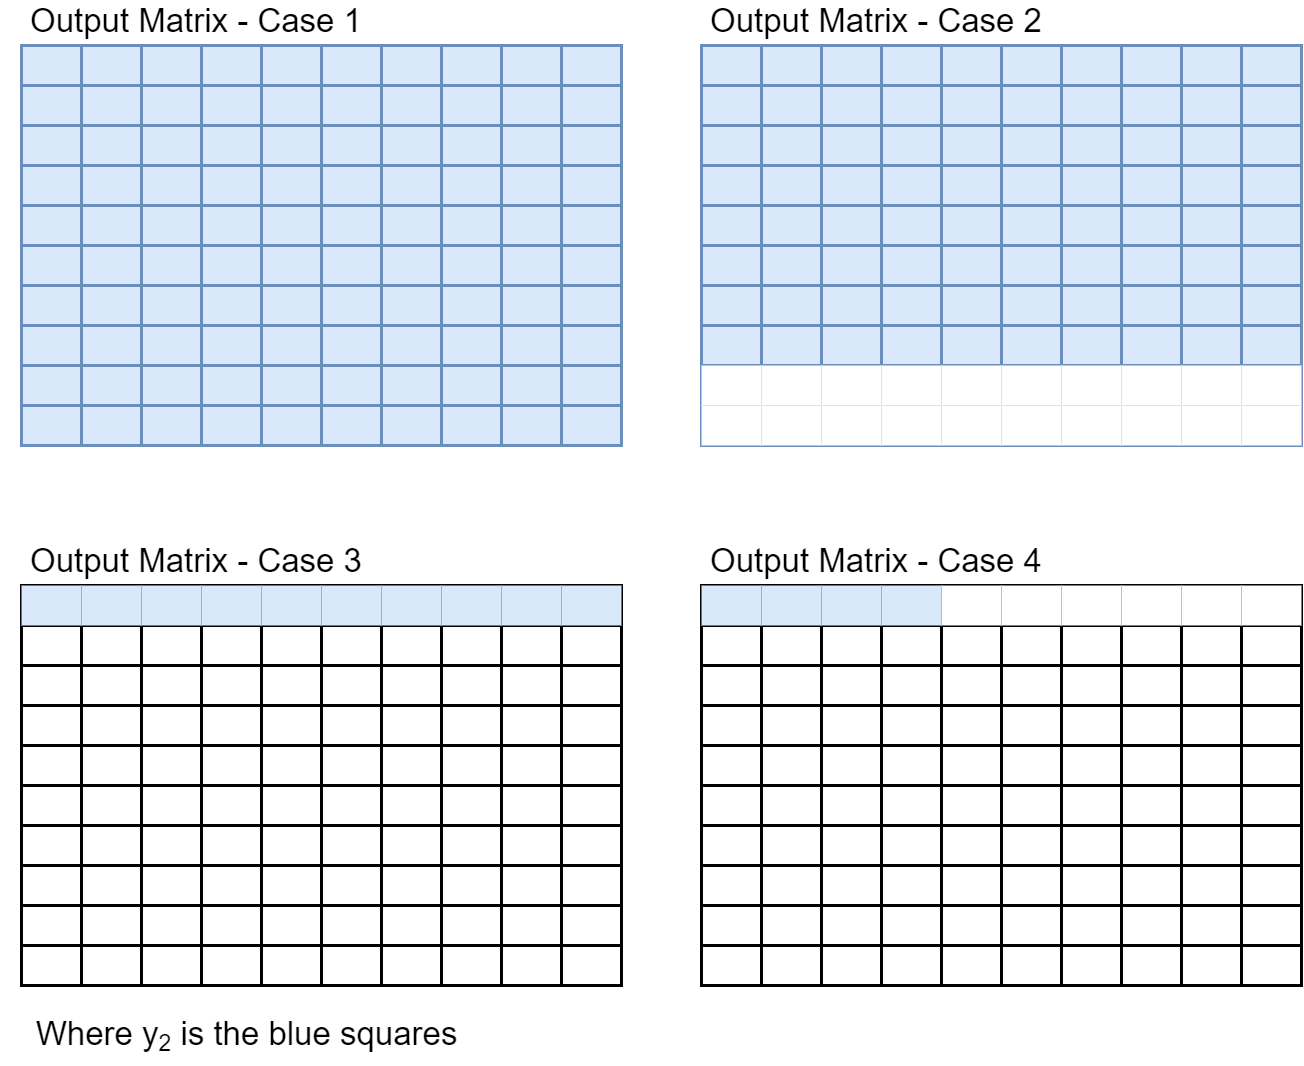
\includegraphics[width=0.7\textwidth]{Figures/Variables.drawio.png}
    \caption{Convolution Scenarios that Versat will have}
    \label{ConvScenarioss}
\end{figure}

The different hardware configurations and the endless possibilities for convolutions mean that all options are covered. 
The only limitation of this generic function is to make partial results which is the last case where the mem can't handle enough inputs for one output.

In Figure~\ref{ConvFlowChart}, the flowchart of each case is presented.

\newpage
\begin{figure}[!htbp]
    \centering
    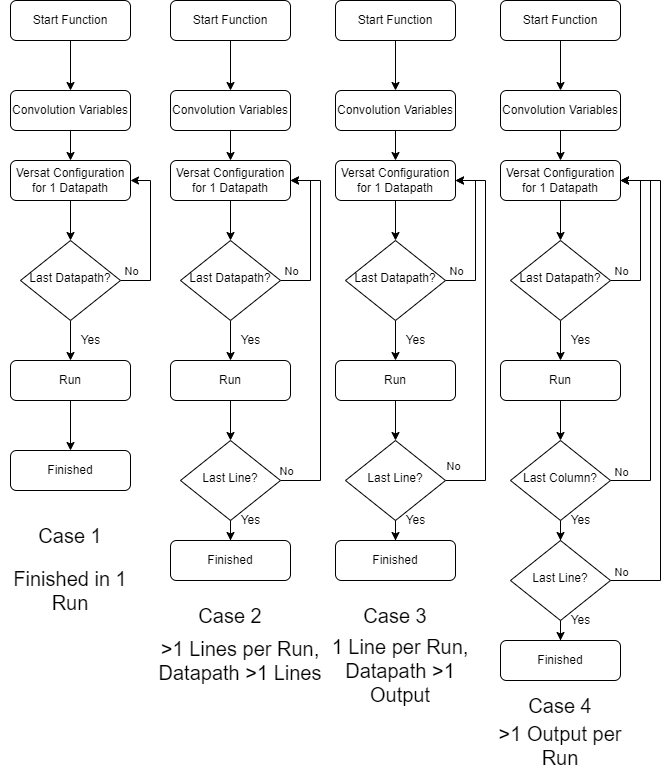
\includegraphics[width=0.65\textwidth]{Figures/ConvolutionFlowChart.drawio.png}
    \caption{Configuration Flowchart for the different scenarios}
    \label{ConvFlowChart}
\end{figure} 

And on Listing\ref{listing:convfinal} the AGU configurations of the VIs that hold the input matrix, the MAC configuration, and finally
the VO AGU configuration.

\lstinputlisting[label=listing:convfinal,language=C++,frame=single,breaklines=true,firstline=449,lastline=478,caption=Versat configurations for one datapath]{./Code/versat_configurations.cpp}


 % add new .tex files for new chapters
\cleardoublepage


%\input{Thesis_new_file} % add new .tex files for new chapters
% \cleardoublepage

%%%%%%%%%%%%%%%%%%%%%%%%%%%%%%%%%%%%%%%%%%%%%%%%%%%%%%%%%%%%%%%%%%%%%%%%
%                                                                      %
%     File: Thesis_Results.tex                                         %
%     Tex Master: Thesis.tex                                           %
%                                                                      %
%     Author: Andre C. Marta                                           %
%     Last modified:  2 Jul 2015                                      %
%                                                                      %
%%%%%%%%%%%%%%%%%%%%%%%%%%%%%%%%%%%%%%%%%%%%%%%%%%%%%%%%%%%%%%%%%%%%%%%%

\chapter{Results}
\label{chapter:results}

In this chapter, the results from the simulator are presented and the new functions developed
for Versat. In Section \ref{section:simtest}, a setup used by a testbench used by DeepVersat is used
to prove the simulator is working according to predictions. Afterward, in section \ref{section:testgencov}, 
a testbench is prepared to test the matrix multiplication and generic convolution with several hardware configurations
available to test the performance of different scenarios in the simulator.

The tests were executed on a 64-bit machine, with an AMD Ryzen 7 5800H Processor and 16GB of RAM running
Windows 11, version 22H2, WSL 2.0 with the image of Ubuntu 20.04. The compiler used is g++ version 9.4.0.

%%%%%%%%%%%%%%%%%%%%%%%%%%%%%%%%%%%%%%%%%%%%%%%%%%%%%%%%%%%%%%%%%%%%%%%%
\section{Simulator Testing}
\label{section:simtest}

To test the simulator, a testbench was created that will create a random input matrix of 5x5
with a kernel size of 3. For each Stage defined in the headers file, a channel will be added and
the result of the convolution will propagate through the stages.

To be more specific in the beginning, the configurations of the VIs are written to transfer the data
from the program to Versat. The data uses the rand() function with seed using current time
so the result is different every time. Both the input matrix and kernel map are randomized.
The former value varies from -25 to 25 while the kernel varies from -5 to 5. Using the data, 
we calculate the result of the convolution in the CPU. Afterward, the configuration for the Bias mem
is done and then stage by stage the configuration of the VI, MAC, and ALU is done. Finally, the
configuration of the VO is written.

\begin{figure}[!htbp]
    \centering
    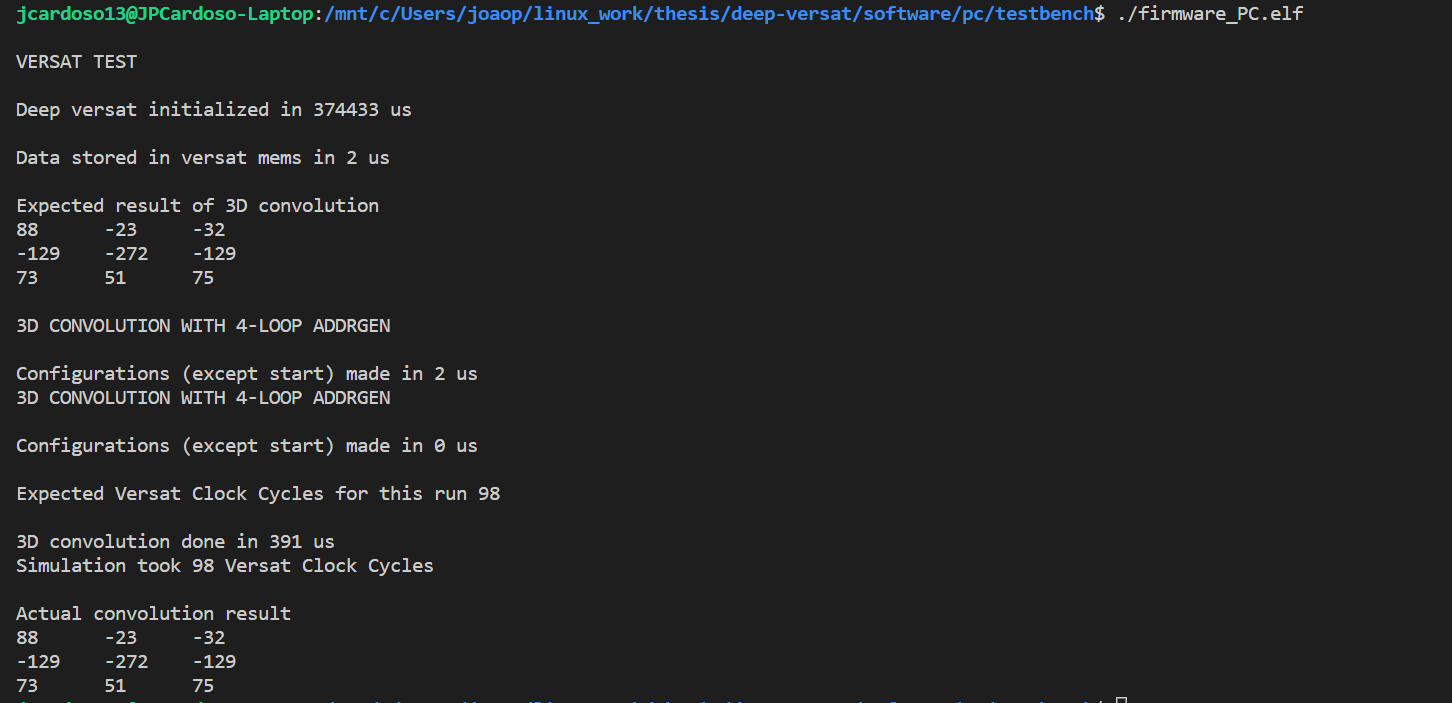
\includegraphics[width=\textwidth]{Figures/test1.png}
    \caption{Simulator test output in terminal}
    \label{figure:test1}
\end{figure} 

The estimated iterations needed are the following:

\[ Est=Delay+Iter_2*Per_2*Iter_1*Per_1\]

Where these are the AGU configurations of the VO where the results are written. The Delay is accumulated
through the several stages by adding two due to the MACs and ALUs.

%%%%%%%%%%%%%%%%%%%%%%%%%%%%%%%%%%%%%%%%%%%%%%%%%%%%%%%%%%%%%%%%%%%%%%%%
\section{Testing the new API}
\label{section:testgencov}

In this section, the same method for the previous testbench is made. 
While the previous one relies on using API v1 for the configuration, these test benches
run the new API. 

\subsection{Testbench for Matrix Multiplication}

The Matrix Multiplication is a quite simple program. The only thing needed is an instance
Versat, run versat\_init(), create the matrixes, and then use the function matrix\_multiplication()
The data is also computed in the CPU the result to verify the output which can be found in
figure \ref{figure:test2}.

\begin{figure}[!htbp]
    \centering
    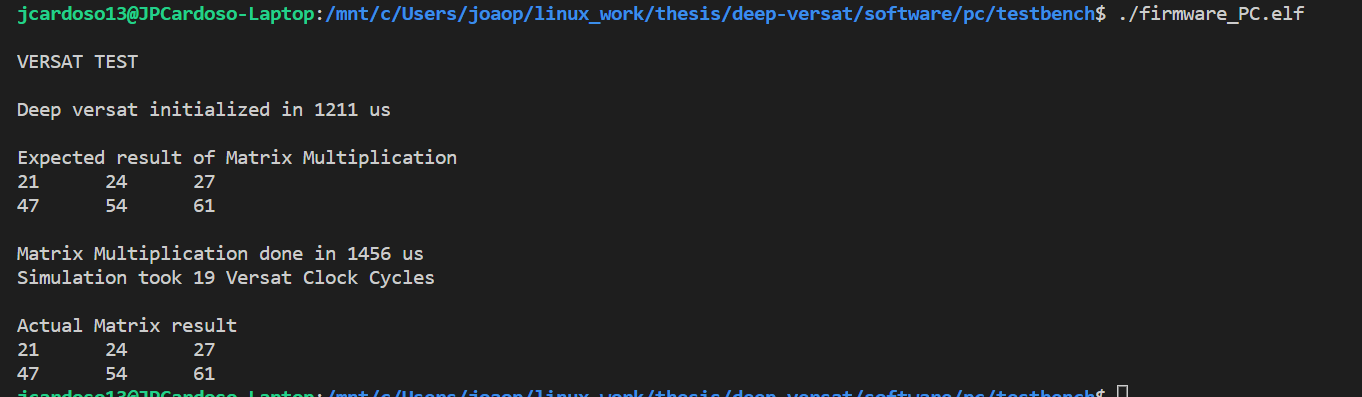
\includegraphics[width=\textwidth]{Figures/test2.png}
    \caption{Matrix Multiplication Testbench Outputs}
    \label{figure:test2}
\end{figure}

\subsection{Testbench for Generic Convolution}

Using the same method on the previous test benches, the following Convolution Layer was used
with several Versat Configurations.

\begin{table}[!htpb]
    \centering
    \begin{tabular}{ll}
    \hline
    \textbf{CNN Variable} & \textbf{Value}        \\ \hline
    Kernel Size            & 2                 \\
    Channels            & 2                       \\
    Number of Kernels            & 2                       \\
    Input Height                  & 12                        \\
    Input Width                & 12                  \\
    Stride              & 1                     \\
    Out Width               & 11                      \\
    Out Height            & 11  \\
    Out Channels                   & 2                     \\ \hline
    \end{tabular}
    \label{table:convInput}
    \caption{CNN Layer on the testbench}
\end{table}

With this layer, figure \ref{figure:test3} has the output result of the generic convolution testbench.
For this specific Versat hardware configuration the number of iterations needed is 711 using 3 Datapaths.

\begin{figure}[!htbp]
    \centering
    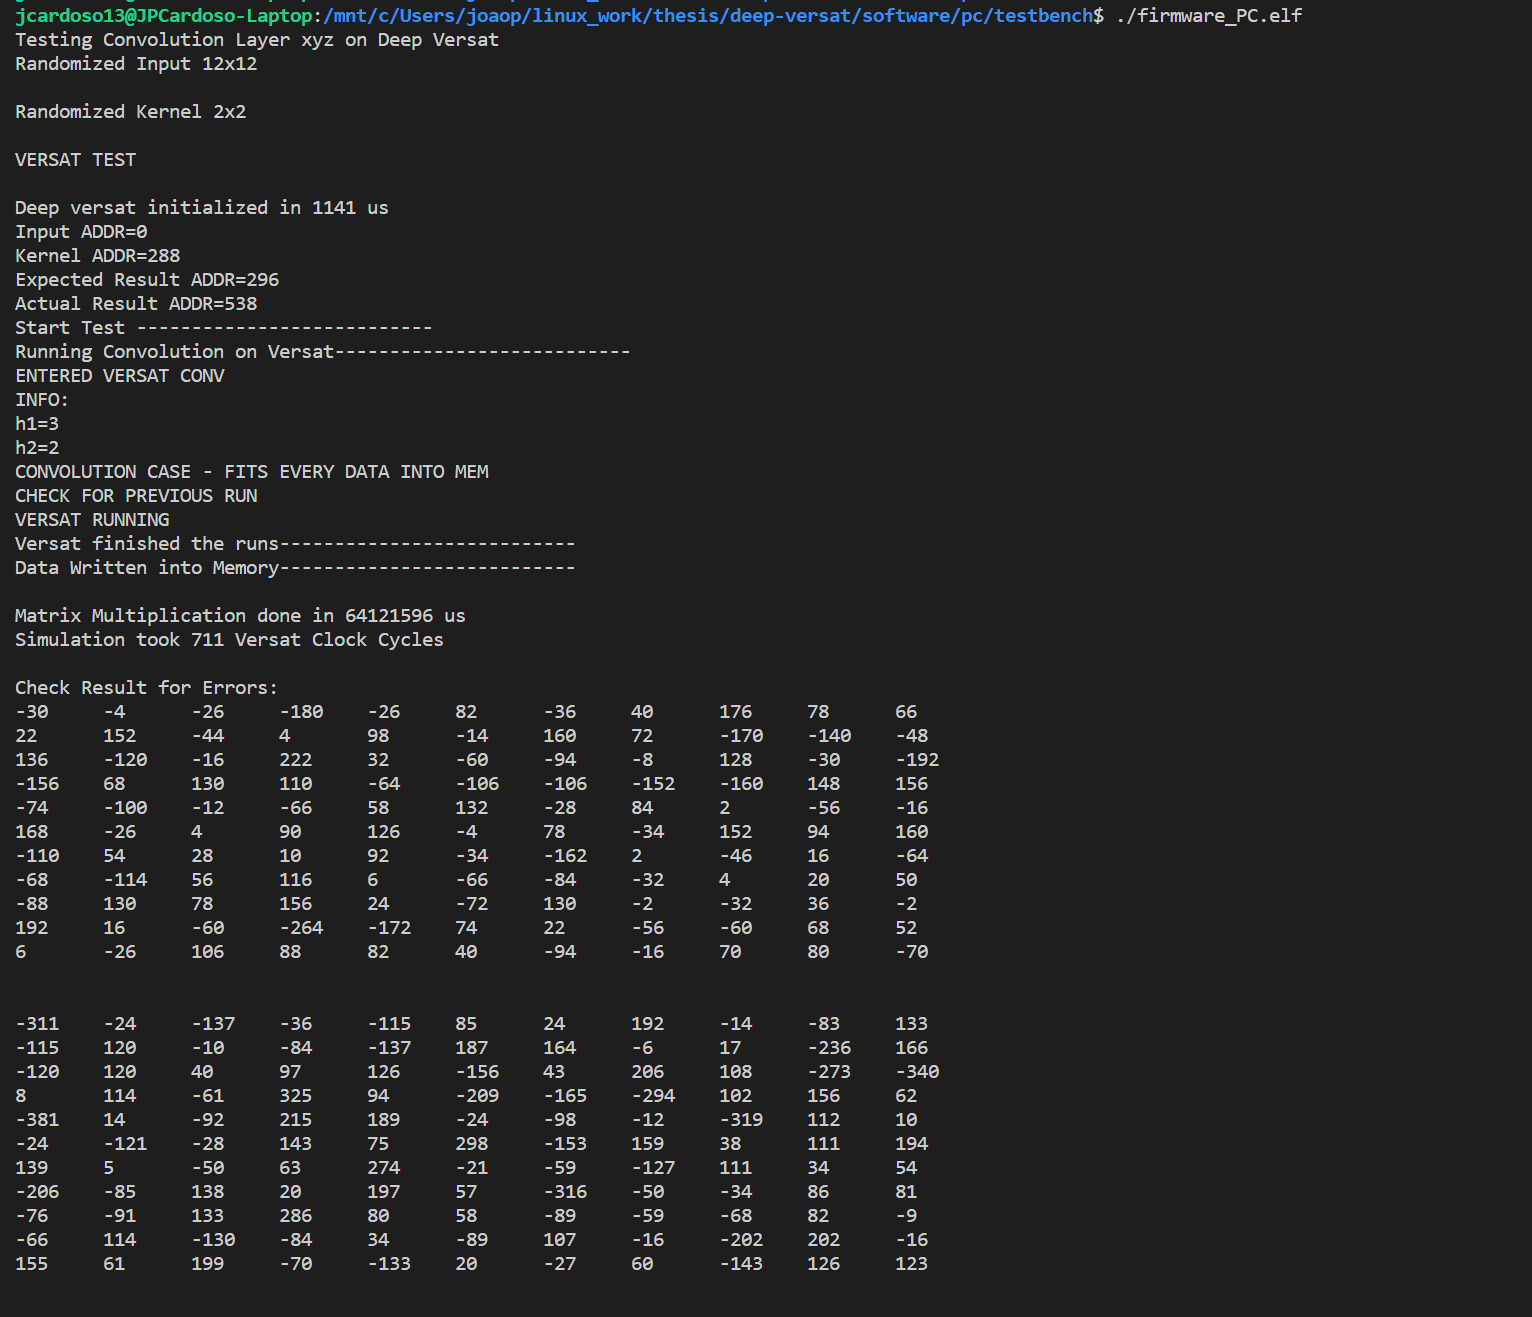
\includegraphics[width=\textwidth]{Figures/test3.png}
    \caption{Generic Convolution Testbench Outputs}
    \label{figure:test3}
\end{figure}

In Table \ref{table:Iterations}, the different Datapath numbers and how it affects performance.
A datapath is a combination of 1 VI, 1 MAC, and 1 VO. So the lower number in the Versat configuration file
decides the number of valid datapaths, of course, VI needs +1 in numbers more than the functional units due to the Kernel memory.
\newpage
\begin{table}[!htpb]
    \centering
    \begin{tabular}{ll}
    \hline
    \textbf{Number of Datapaths} &  \textbf{Iterations}        \\ \hline
    1          & 1943                 \\
	2          & 1063                 \\
	3          & 711                 \\
	4          & 535                 \\
	6          & 359                 \\
	8          & 359                 \\
	11          & 183                 \\
	16          & 183                 \\
    22            & 183                       \\  \hline
    \end{tabular}
    \label{table:Iterations}
    \caption{CNN Layer on the testbench with several Versat hardware configurations}
\end{table}

The reason for these results is quite simple. In total, 11 output lines are divided
by the datapaths. When the division is not a whole number, the remainder gets distributed
by available datapaths. The consequence of this, when changing from 6 to 8 datapaths, the performance
doesn't get any better. Datapath 0 will have to run twice to (2 lines) while Datapath 8 will run 1 line.
To increase further the performance, the output channels would have to be divided through more datapaths. % file "Thesis_Results.tex"
\cleardoublepage

%%%%%%%%%%%%%%%%%%%%%%%%%%%%%%%%%%%%%%%%%%%%%%%%%%%%%%%%%%%%%%%%%%%%%%%%
%                                                                      %
%     File: Thesis_Conclusions.tex                                     %
%     Tex Master: Thesis.tex                                           %
%                                                                      %
%     Author: Andre C. Marta                                           %
%     Last modified:  2 Jul 2015                                      %
%                                                                      %
%%%%%%%%%%%%%%%%%%%%%%%%%%%%%%%%%%%%%%%%%%%%%%%%%%%%%%%%%%%%%%%%%%%%%%%%

\chapter{Conclusions}
\label{chapter:conclusions}

In this thesis, a compiler and software simulation model for Deep Neural
Networks running on the DeepVersat Architecture are presented. The simulator
runs orders of magnitude faster than an RTL simulator, allowing for the fast
testing of new software configurations and workloads. It can accurately predict the
performance of the workloads running on DeepVersat. These tools are helpful for
architectural exploration, helping to determine the number of functional units,
stages, or memory sizes needed for optimal performance.


% ----------------------------------------------------------------------
\section{Achievements}
\label{section:achievements}

First, a darknet framework for embedded devices and new tools have been
developed to parse CFG, which are essential for future work using the Versat
CGRA. These tools make running any CNN on embedded hardware possible, even if
it comprises just a CPU.

Second, a software simulation model, referred to as the simulator, has been
developed and can emulate the hardware output. A new program was written for
Versat can be compiled in seconds instead of the several minutes it takes to
compile the DeepVersat FPGA bitstream.

Third, a generic convolution method has been developed to run any 
convolution layer efficiently. Changing the Versat
parameters allows a new hardware convolution configuration to be tested, and the
performance can be determined with the simulator.

Lastly, a new Versat API has been developed, which can make writing code for
Versat is akin to writing regular C++ code that runs on a CPU.


% ----------------------------------------------------------------------
\section{Future Work}
\label{section:future}

For future work, prominent sections need to be addressed. For example, while developing darknet lite,
they were not linked with Versat and the simulator. For that, a max pool generic function
must be added and redirect the convolution layer to the generic convolution for Versat.

Other work includes improving the simulator by adding new FUs and generic functions. On that
adding partial results to the convolution will also benefit possible Versat configurations.

Versat is a highly versatile CGRA, but for deep neural networks, datapath width is needed, i.e.
more memories and MACs to add more MACs means increasing the propagation time and, as such, grouping VIs and MACs into a bigger functional unit to avoid the usage of a multiplexer at the entrance of the MACs. This could be called the SIMD path, while the rest of the configuration
could still be highly configurable and have the standard functional units to have the cake and eat it too.
Highest performance and high configurability.

On the memory side, the ability to configure the size of each mem would give more flexibility
and the configurations to be more data efficient. For example, in this thesis, there were two types of VIs. One
that holds the inputs and another that contains the kernels. The kernels don't use much space, and thus
the memory will hold a lot of empty values because both VIs have the same size.


 % file "Thesis_Conclusions.tex"
\cleardoublepage

% ----------------------------------------------------------------------
%  Bibliography
% ----------------------------------------------------------------------

% Add entry in the table of contents as chapter
\phantomsection
\addcontentsline{toc}{chapter}{\bibname}

% Include all references in the .bib file, even non-cited ones...
%\nocite{*} % This should be used carefully because it is not correct!

% Produces the bibliography section when processed by BibTeX
%
% Bibliography style
% > entries ordered alphabetically
%\bibliographystyle{plain}
% > unsorted with entries appearing in the order in which the citations appear.
%\bibliographystyle{unsrt}
% > entries ordered alphabetically, with first names and names of journals and months abbreviated
%\bibliographystyle{abbrv}
% > entries ordered alphabetically, with reference markers based on authors' initials and publication year
%\bibliographystyle{alpha}
%
% Replacement bibliography styles provided by 'natbib' package
% (plainnat.bst, abbrvnat.bst, unsrtnat.bst )
% > entries ordered alphabetically
%\bibliographystyle{plainnat}
% > unsorted with entries appearing in the order in which the citations appear.
%\bibliographystyle{unsrtnat}
% > entries ordered alphabetically, with first names and names of journals and months abbreviated
%\bibliographystyle{abbrvnat} % <<<<< SELECT IF USING REFERENCES BY AUTHOR/YEAR
% > entries ordered alphabetically, with reference markers based on authors' initials and publication year
%\bibliographystyle{alpha}
%
% Custom bibliography style adapted from 'natbib' package
%   (based on http://tex.stackexchange.com/questions/5053/is-it-possible-to-get-unsrt-abbrv-bibliography)
%   (unsrtnat.bst + abbrvnat.bst -> abbrvunsrtnat.bst)
%   (original files copied from:
%   http://tug.ctan.org/macros/latex/contrib/natbib/abbrvnat.bst
%   http://tug.ctan.org/macros/latex/contrib/natbib/unsrtnat.bst
% > unsorted with entries appearing in the order in which the citations appear, with first names and names of journals and months abbreviated.
\bibliographystyle{abbrvunsrtnat} % <<<<< SELECT IF USING REFERENCES BY NUMBER (CITATION ORDER)

% External bibliography database file in the BibTeX format
\bibliography{Thesis_bib_DB} % file "Thesis_bib_DB.bib"

\cleardoublepage

% ----------------------------------------------------------------------
%  Appendix (optional)
%
%  CAUTION: 1) the main document (up to the conclusions) shall not exceed 80 pages
%           2) the document shall not exceed a total of 100 pages (per IST regulations)
% ----------------------------------------------------------------------
%\appendix

% add page number prefix according to apendix chapter (optional)
%\renewcommand{\thepage}{\thechapter.\arabic{page}}

% re-set arabic numbering (A.1,A.2,...) (optional, use only if chapter prefix is added)
%\setcounter{page}{1}

%%%%%%%%%%%%%%%%%%%%%%%%%%%%%%%%%%%%%%%%%%%%%%%%%%%%%%%%%%%%%%%%%%%%%%%%%
%                                                                      %
%     File: Thesis_Appendix_A.tex                                      %
%     Tex Master: Thesis.tex                                           %
%                                                                      %
%     Author: Andre C. Marta                                           %
%     Last modified :  2 Jul 2015                                      %
%                                                                      %
%%%%%%%%%%%%%%%%%%%%%%%%%%%%%%%%%%%%%%%%%%%%%%%%%%%%%%%%%%%%%%%%%%%%%%%%

\chapter{Vector calculus}
\label{chapter:appendixVectors}

In case an appendix if deemed necessary, the document cannot exceed a total of 100 pages...

Some definitions and vector identities are listed in the section below.

% ----------------------------------------------------------------------
\section{Vector identities}
\label{section:vectorIdentities}

\begin{equation}
	\nabla \times \left( \nabla \phi \right) = 0
	\label{eq:cross_nnp}
\end{equation}

\begin{equation}
	\nabla \cdot \left( \nabla \times {\bf u} \right) = 0
	\label{eq:dotCross_nnu}
\end{equation}

 % file "Thesis_Appendix_A.tex"
%\cleardoublepage

% re-set arabic numbering (B.1,B.2,...) (optional, use only if chapter prefix is added)
%\setcounter{page}{1}

%%%%%%%%%%%%%%%%%%%%%%%%%%%%%%%%%%%%%%%%%%%%%%%%%%%%%%%%%%%%%%%%%%%%%%%%%
%                                                                      %
%     File: Thesis_Appendix_B.tex                                      %
%     Tex Master: Thesis.tex                                           %
%                                                                      %
%     Author: Andre C. Marta                                           %
%     Last modified :  2 Jul 2015                                      %
%                                                                      %
%%%%%%%%%%%%%%%%%%%%%%%%%%%%%%%%%%%%%%%%%%%%%%%%%%%%%%%%%%%%%%%%%%%%%%%%

\chapter{Technical Datasheets}
\label{chapter:appendixDatasheets}

It is possible to add PDF files to the document, such as technical sheets of some equipment used in the work.

% ----------------------------------------------------------------------
\section{Some Datasheet}
\label{section:datasheet}

% See more options to include PDF files in
% http://mirror.unl.edu/ctan/macros/latex/contrib/pdfpages/pdfpages.pdf
\includepdf[pages={1-2},nup=1x2,landscape=true]{Figures/SolarCell_Sunpower_C60.pdf}

 % file "Thesis_Appendix_B.tex"
%\cleardoublepage

% ----------------------------------------------------------------------
\end{document}
% ----------------------------------------------------------------------

